\documentclass[10pt,twoside,notitlepage]{report}
%\usepackage[utf8]{inputenc}
%\usepackage[a4paper,width=150mm,top=25mm,bottom=25mm,bindingoffset=6mm,headsep=1cm,headheight=2cm]{geometry}
\usepackage[a4paper, margin=2.5cm]{geometry}
\usepackage{setspace}
\usepackage{pgfplots}
%\pgfplotsset{compat=newest}
%\usepgfplotslibrary{fillbetween}
\linespread{1.25}
\usepackage{float}
\usepackage{amsfonts,latexsym,amsthm,amssymb,amsmath,amscd,euscript,graphicx,subfig, tikz-cd,bbm}
\usepackage{framed}
\usepackage{fullpage}
\usepackage{hyperref}
    \hypersetup{colorlinks=true,citecolor=blue,urlcolor =black,linkbordercolor={1 0 0}}
\usepackage{enumitem}
\usepackage{esint}
\usepackage[backend=biber, style=alphabetic]{biblatex}
\usepackage{amssymb}
\addbibresource{references.bib}

\usepackage{titling}
\usepackage{titlesec}
\usepackage{caption}
\usepackage{float}
\titleformat{\chapter}[display]   
{\normalfont\huge\bfseries}{\chaptertitlename\ \thechapter}{20pt}{\Huge}   
\titlespacing*{\chapter}{0pt}{-30pt}{40pt}

\graphicspath{ {images/} }

\theoremstyle{plain}
\newtheorem{thm}{Theorem}[section]
\newtheorem{clm}[thm]{Claim}
\newtheorem*{clm*}{Claim}
\newtheorem{lem}[thm]{Lemma}
\newtheorem*{lem*}{Lemma}
\newtheorem{cor}[thm]{Corollary}
\newtheorem*{cor*}{Corollary}
\newtheorem{prop}[thm]{Proposition}
\newtheorem*{prop*}{Proposition}
\newtheorem{conj}[thm]{Conjecture}
\newtheorem{rmk}{Remark}[section]
\newtheorem*{rmk*}{Remark}
\newtheorem{note}{Note}[section]
\newtheorem*{note*}{Note}



\theoremstyle{definition}
\newtheorem{defn}{Definition}[section]
\newtheorem{exmp}{Example}[section]
\newtheorem{nexmp}[exmp]{Non-example}


\newcommand{\R}{\mathbb{R}}
\newcommand{\N}{\mathbb{N}}
\newcommand{\NN}{\mathcal{N}}
\newcommand{\Z}{\mathbb{Z}}
\newcommand{\C}{\mathbb{C}}
\newcommand{\Q}{\mathbb{Q}}
\newcommand{\T}{\mathbb{T}}
\newcommand{\FF}{\mathcal{F}}
\newcommand{\TT}{\mathcal{T}}
\newcommand{\I}{\mathbb{I}}
\newcommand{\PP}{\mathbb{P}}
\newcommand{\Pcal}{\mathcal{P}}
\newcommand{\e}{\varepsilon}
\newcommand{\w}{\omega}
\newcommand{\topO}{\mathcal{O}}
\newcommand{\1}{\mathbbm{1}}
\newcommand{\Scal}{\mathcal{S}}
\newcommand{\dd}{\mathrm{d}}
\newcommand{\calU}{\mathcal{U}}  %Box in space
\newcommand{\freqU}{\calU^\circ} % Box in frequency
\newcommand{\Part}{\mathcal{P}} % Power set
\newcommand{\Dec}{\mathcal{D}} %decoupling constant 
\newcommand{\BilinDec}{\mathcal{B}} %bilinear decoupling constant 
\newcommand{\nc}{\newcommand}
\newcommand{\scale}[1]{\delta^{\left(\frac{k}{k+1}\right)^{#1}}}
\newcommand{\scaleinv}{\delta^{-\varepsilon k/(k+1)varepsilon}}
\nc{\on}{\operatorname}
\newcommand{\supp}{\text{supp}}
\newcommand{\dist}{\text{dist}}
\newcommand{\intslash}{\mathrlap{\int}\hspace{0.5em}\bigg{/} \int}
\newcommand{\lpl}{L^{p_l}(\R^l)}


\DeclareMathOperator{\img}{img}
\DeclareMathOperator{\nul}{null}
\DeclareMathOperator{\esup}{ess\,sup}
\DeclareMathOperator{\mat}{mat}
\DeclareMathOperator{\lcm}{lcm}

\usepackage{mathtools}
\newcommand{\defeq}{\vcentcolon=}
\newcommand{\eqdef}{=\vcentcolon}
\newcommand{\nsub}{\trianglelefteq}
\DeclarePairedDelimiter\ceil{\lceil}{\rceil}
\DeclarePairedDelimiter\floor{\lfloor}{\rfloor}
\DeclarePairedDelimiter\abs{\lvert}{\rvert}
\DeclarePairedDelimiter\norm{\lVert}{\rVert}
\DeclarePairedDelimiter\inner{\langle}{\rangle}

\newcommand\SetSymbol[1][]{%
\nonscript\:#1\vert
\allowbreak
\nonscript\:
\mathopen{}}
\DeclarePairedDelimiterX\Set[1]\{\}{\renewcommand\given{\SetSymbol[\delimsize]}#1}
\DeclarePairedDelimiterXPP\EE[1]{\E}{\lparen}{\rparen}{}{\renewcommand\given{\SetSymbol[\delimsize]}#1} % Conditional expectation \EE{ f \given A }
\DeclarePairedDelimiterX\inn[2]{\langle}{\rangle}{#1,#2}
\def\biginn#1#2{\inn[\big]{#1}{#2}}

\makeatletter
\let\oldabs\abs
\def\abs{\@ifstar{\oldabs}{\oldabs*}}
%
\let\oldnorm\norm
\def\norm{\@ifstar{\oldnorm}{\oldnorm*}}
\let\oldinner\inner
\def\inner{\@ifstar{\oldinner}{\oldinner*}}
\makeatother



\begin{document}
%\chapter{Parabola}
\chapter{The parabola case}
In this chapter, our aim is to introduce some of the fundamental concepts and ideas underlying the proof of the $\ell^2$-decoupling in the two-dimensional case.
Our presentation draws heavily from sources, including the original work by Bourgain and Demeter [BD14], and the most recent proof for the parabola which can be seen as a particular case of [Short Proof].

On the first half of this chapter we present what is known as the bilinear Reduction which allows us to transform our problem into a multilinear one, this observation is the first major driving force of the proof and here we follow a curated 
version of the original work, see [DEM17]. For the later half we present some techniques used in [Short Proof] resorting to some heuristics of the Fourier transform which allows us to see the second driving force of the proof from a geometrical 
perspective, this is the content of subsections \ref{subsection:Wave packet approach} and \ref{subsection:Averaging approach}.

The choice to deviate from the original work is two-fold. Following [BD14], the analogous version of subsection \ref{section:bootstrap} isn't that more complicated, however since we are interested in proving the analogous problem for the moment 
curve this approach won't accomplish that, so this nicely sets up the work for Chapter 2 and allows us to more easily see the geometric aspect of the decoupling problems.

\newpage
\section{Parabola} 
Consider the subset of the parabola above $[0,1]$, parameterized in the usual way, $$\Gamma(t)=(t,t^2)\text{, }t\in[0,1].$$ For $\delta \in (0,1)$, let $\Part(\delta)$ denote the partition of the interval $[0,1]$ into dyadic intervals with length $2^{-\lceil \log_2 \delta^{-1} \rceil}$.
For a dyadic interval $J$, let $\calU_{J}$ be the parallelepiped of dimensions $\abs{J}^{1} \times \abs{J}^{2}$ whose center is $\Gamma(c_J)$ and sides are parallel to $\partial^{1}\Gamma(c_{J})$, $\partial^{2}\Gamma(c_{J})$, where $c_J$ is the center of $J$.
We write $\norm{\cdot}_{6} := \norm{\cdot}_{L^{6}(\R^{2})}$.
\begin{center}
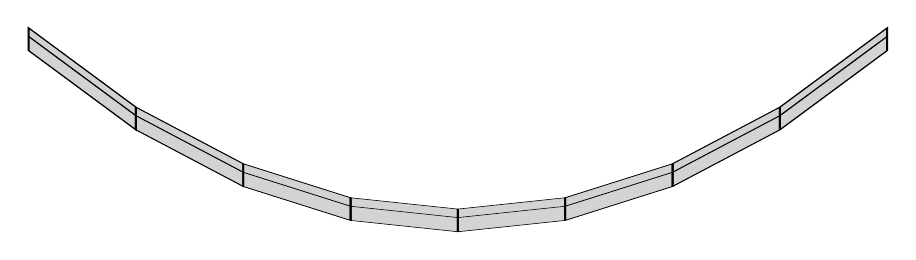
\begin{tikzpicture}[scale=0.5,xscale=3.5]

\definecolor{darkgray176}{RGB}{176,176,176}
\definecolor{lightgray}{RGB}{211,211,211}

\begin{axis}[
hide x axis,
hide y axis,
tick align=outside,
tick pos=left,
x grid style={darkgray176},
xmin=-1.1, xmax=1.1,
xtick style={color=black},
y grid style={darkgray176},
ymin=-0.134375, ymax=1.103125,
ytick style={color=black}
]
\path [draw=lightgray, fill=lightgray]
(axis cs:-1,0.921875)
--(axis cs:-0.75,0.484375)
--(axis cs:-0.75,0.609375)
--(axis cs:-1,1.046875)
--cycle;
\path [draw=lightgray, fill=lightgray]
(axis cs:-0.75,0.484375)
--(axis cs:-0.5,0.171875)
--(axis cs:-0.5,0.296875)
--(axis cs:-0.75,0.609375)
--cycle;
\path [draw=lightgray, fill=lightgray]
(axis cs:-0.5,0.171875)
--(axis cs:-0.25,-0.015625)
--(axis cs:-0.25,0.109375)
--(axis cs:-0.5,0.296875)
--cycle;
\path [draw=lightgray, fill=lightgray]
(axis cs:-0.25,-0.015625)
--(axis cs:0,-0.078125)
--(axis cs:0,0.046875)
--(axis cs:-0.25,0.109375)
--cycle;
\path [draw=lightgray, fill=lightgray]
(axis cs:0,-0.078125)
--(axis cs:0.25,-0.015625)
--(axis cs:0.25,0.109375)
--(axis cs:0,0.046875)
--cycle;
\path [draw=lightgray, fill=lightgray]
(axis cs:0.25,-0.015625)
--(axis cs:0.5,0.171875)
--(axis cs:0.5,0.296875)
--(axis cs:0.25,0.109375)
--cycle;
\path [draw=lightgray, fill=lightgray]
(axis cs:0.5,0.171875)
--(axis cs:0.75,0.484375)
--(axis cs:0.75,0.609375)
--(axis cs:0.5,0.296875)
--cycle;
\path [draw=lightgray, fill=lightgray]
(axis cs:0.75,0.484375)
--(axis cs:1,0.921875)
--(axis cs:1,1.046875)
--(axis cs:0.75,0.609375)
--cycle;
\addplot [line width=0.4pt, black]
table {%
-1 1
-0.75 0.5625
-0.5 0.25
-0.25 0.0625
0 0
0.25 0.0625
0.5 0.25
0.75 0.5625
1 1
};
\addplot [line width=0.4pt, black]
table {%
-1 0.921875
-0.75 0.484375
-0.75 0.609375
-1 1.046875
-1 0.921875
};
\addplot [line width=0.4pt, black]
table {%
-0.75 0.484375
-0.5 0.171875
-0.5 0.296875
-0.75 0.609375
-0.75 0.484375
};
\addplot [line width=0.4pt, black]
table {%
-0.5 0.171875
-0.25 -0.015625
-0.25 0.109375
-0.5 0.296875
-0.5 0.171875
};
\addplot [line width=0.4pt, black]
table {%
-0.25 -0.015625
0 -0.078125
0 0.046875
-0.25 0.109375
-0.25 -0.015625
};
\addplot [line width=0.4pt, black]
table {%
0 -0.078125
0.25 -0.015625
0.25 0.109375
0 0.046875
0 -0.078125
};
\addplot [line width=0.4pt, black]
table {%
0.25 -0.015625
0.5 0.171875
0.5 0.296875
0.25 0.109375
0.25 -0.015625
};
\addplot [line width=0.4pt, black]
table {%
0.5 0.171875
0.75 0.484375
0.75 0.609375
0.5 0.296875
0.5 0.171875
};
\addplot [line width=0.4pt, black]
table {%
0.75 0.484375
1 0.921875
1 1.046875
0.75 0.609375
0.75 0.484375
};
\end{axis}

\end{tikzpicture}
\end{center}
\begin{defn}\label{def:dec-const}
For $\delta \in (0,1)$, the \emph{$\ell^{2}L^{6}$ decoupling constant} $\Dec(\delta)$ for the parabola is the smallest number for which the inequality
\begin{equation}
\label{eq:dec-const}
\norm{ \sum_{J \in \Part(\delta)} f_{J} }_{p_{k}}
\leq \Dec(\delta)
\Bigl( \sum_{J \in \Part(\delta)} \norm{ f_{J} }_{p_{k}}^{2} \Bigr)^{1/2}
\end{equation}
holds for any tuple of functions $(f_{J})_{J \in \Part(\delta)}$ with $\text{supp} \widehat{f_{J}} \subseteq \calU_{J}$ for all $J$.
\end{defn}

\begin{thm}[BD14]\label{thm:main}
For every $\epsilon>0$, there exists a finite constant $C_{\epsilon}$ such that
\begin{equation}
\label{eq:main}
\Dec(\delta) \le C_{\epsilon} \delta^{-\epsilon}, \text{ for every } \delta\in (0, 1).
\end{equation}
\end{thm}


In the original work, the authors proved Theorem \ref{thm:main} by working with a slightly different geometry in the frequency domain. They considered a $\delta^2$-neighborhood of the parabola, denoted by $\mathcal{N}(\delta)\defeq \{(t,t^2+s)\mid t\in[0,1], s\in[0,\delta^2]\}$, partitioned it into almost rectangular boxes $\theta_{J}\defeq\{(t,t^2+s)\mid t\in J, s\in[0,\delta^2]\}$ and considered $(f_{J})_{J \in \Part(\delta)}$ with $\text{supp} \widehat{f_{J}} \subseteq \theta_{J}$ for all $J$ in Definition \ref{def:dec-const}. Let's call $\mathfrak{D}(\delta)$ the \emph{$\ell^{2}L^{6}$} decoupling constant for the curved partition.

We can easily see $\mathfrak{D}(\delta)\lesssim \Dec(\delta)$ by the following picture,
\begin{center}
\begin{tikzpicture}[scale=2]
\begin{axis}[
    hide axis,
    enlarge x limits=0.8, % Add horizontal margin
    enlarge y limits=0.8  % Add vertical margin
    ]

% Plot 1
\addplot [name path = A,
    domain = 0:0.45] {x^2+0.1};

% Plot 2
\addplot [name path = B,
    domain = 0:0.45] {x^2};

 %plot3
\addplot [name path = C,
    domain = 0:0.45] {x^2-0.1};

\addplot [black!20] fill between [of = A and C, soft clip={domain=0:0.45}];

%draw left points of parallelogram
\draw (0,-0.1-0.05) -- (0,0.1);

%draw right points of parallelogram
\draw (0.45,0.45^2+0.1) -- (0.45,0.45^2-0.1-0.05);

\draw (0,-0.1-0.05) -- (0.45,0.45^2-0.1-0.05);
\draw (0,0.1) -- (0.45,0.45^2+0.1);

% Add curly brackets for side lengths
\draw[decorate,decoration={brace,amplitude=5pt,mirror}] (0,-0.1-0.08) -- node[below=6pt] {$\sim \delta$} (0.45,0.45^2-0.1-0.08);
\draw[decorate,decoration={brace,amplitude=5pt}] (0.47,0.45^2+0.1) -- node[right=6pt] {$\sim \delta^2$} (0.47,0.45^2-0.1-0.05);

\draw[dashed] (0,-0.1-0.05) -- (0,-0.3); % Starting at (0,-0.1-0.05)
\draw[dashed] (0.45,0.45^2-0.1-0.05) -- (0.45,-0.3); % Starting at 
% Add the bold, thicker, labeled line "I" at the center
\draw[thick, |-|] (0-0.005,-0.3) -- node[below=8pt] {$J$} (0.45+0.005,-0.3);

\end{axis}
\end{tikzpicture}
\end{center}

 Working with this weaker condition is also motivated by the higher-dimensional case where this kind of anisotropic box works well under certain changes of variables.

A crucial component underlining all decoupling proof is the idea that we can rescale the problem and preserve the decoupling property. In the context of the parabola, this idea starts with following observation, let $I =\left[a,a+\eta \right]$ and let $A_I: \mathbb{R}^2 \longrightarrow \mathbb{R}^2$, defined by 

$$
A_I(x_1,x_2) = \begin{pmatrix}
a \\
a^2
\end{pmatrix} +
\begin{pmatrix}
\eta & 0 \\
2a\eta & \eta^2
\end{pmatrix} 
\begin{pmatrix}
x_1 \\
x_2
\end{pmatrix}
$$
then $A_I \Gamma(t)= \Gamma(a+t\eta)$ for $t\in\R$, in particular one maps $\Gamma(I)$ to the whole curve via $A_I^{-1}$. Furthermore, this map preserves the geometry of the frequency space, i.e, for dyadic intervals $I,J$ with $J \subseteq I \subseteq [0,1]$, we have
\[
A_I^{-1} \calU_{J} = \calU_{J_I},
\]
where $J_I := \eta^{-1} (J - a)$ if $I = [a,a+\eta]$. To see why this is true, combine the relation
$$
(DA_I) \partial^i \Gamma(t) = \kappa^i (\partial^i \Gamma)(a+t\kappa) \quad \text{for all $i\geq 1$ and $t\in\R$}
$$
with the definition of $\calU_J$ (an exemple calculation is done for the full moment curve).
\begin{lem}(Monotony of decoupling constant)
Given $0<\delta_L \leq \delta_S \leq 1$, $\Dec(\delta_L)\leq \Dec(\delta_S)$.
\end{lem}
\begin{proof}
\begin{equation}
    \sum_{J \in \Part(I,\delta_L)} \norm{ f_{J} }_{6}^{2} = \sum_{J \in \Part(I,\delta_L)}\sum_{J^{\prime} \in \Part(J,\delta_S)} \norm{ f_{J^{\prime}} }_{6}^{2},
\end{equation}
apply $\ell^2(\Part(J,\delta_S)) \leq \#\Part(J,\delta_S)\, \ell^6(\Part(J,\delta_S))$ and sum to obtain
\begin{equation}\label{eq:monotony }
    \lesssim \delta_S ^{1-\frac{1}{3}}\sum_{J \in \Part(I,\delta_L)} \norm{ f_{J^{\prime}} }_{6}^{2} \leq \sum_{J \in \Part(I,\delta_L)} \norm{ f_{J^{\prime}} }_{6}^{2}.
\end{equation}
Combine \ref{eq:monotony } with Definition \ref{defn:dec-const} to get the desired conclusion.
\end{proof}
\begin{lem}(Parabolic rescaling) \label{lem:lin_rescale}
Let $I \in \Part(2^{-n})$ for some integer $n \geq 0$.
For any $\delta \in (0,2^{-n})$ and any tuple of functions $(f_J)_{J \in \Part(I,\delta)}$ with $\supp  \widehat{f_J} \subseteq \calU_{J}$ for all $J$, the following inequality holds:
\begin{equation} \label{eq:lin_rescale}
\norm{ f_{I} }_{6}
\leq
\Dec(2^{n} \delta) \Bigl( \sum_{J \in \Part(I, \delta)} \norm{ f_{J} }_{6}^{2} \Bigr)^{1/2}.
\end{equation}
\end{lem}
\begin{proof}
    Suppose that $I = [a,a+2^{-n}]$. For $J \in \Part(I, \delta)$ and $K = J_{I}\in \Part(2^{n}\delta)$, let the function $g_{K}$ be such that  $\widehat{f_{J}} \circ A_{I} = \widehat{g_{K}}$, so that $\supp\,\widehat{g_{K}} \subseteq \calU_{K}=\calU_{J_{I}}$. Applying \ref{eq:dec-const} to the family $(g_{K})$ and changing variables on both sides we obtain \ref{eq:lin_rescale}.
\end{proof}
There's a couple of observation worth noting about this Lemma. Of course one could formulate the analogous decoupling problem for function Fourier supported in $\calU_{I}$, with decoupling constant denoted by $\Dec_{I}(\delta)$. Trivially we could apply Definition \ref{def:dec-const} to the family $(f_J)_{J \in \Part(I,\delta)}$ and obtain
\begin{equation}
\norm{ f_{I} }_{6}
\leq \Dec(\delta)
\Bigl( \sum_{J \in \Part(I,\delta)} \norm{ f_{J} }_{6}^{2} \Bigr)^{1/2}
\end{equation}
which implies $\Dec_{I}(\delta)\leq \Dec(\delta)$. On another hand, Lemma \ref{lem:lin_rescale} implies $\Dec_{I}(\delta)\leq \Dec(2^{n}\delta)$, which can be seen as a stronger bound since, $\Dec(2^{n}\delta)\lesssim \Dec(\delta)$, by monotony. 

\begin{rmk}(Cost of decoupling)
    We can interpret $\Dec(\delta)$ as the cost of decoupling $[0,1]$ into intervals of size $\delta$, \ref{eq:lin_rescale} tells us that the cost of the decoupling $I$ into intervals of size $\delta$, and easier problem, is $\Dec(2^{n} \delta)$. 
\end{rmk}
As an immediate application of parabolic rescaling we have almost multiplicativity of the decoupling constant.

\begin{lem}(Almost multiplicativity)\label{lem:submulti}
    Let $n\in\N$ and $0<\delta<2^{-n}$, then
    $$
    \Dec(\delta) \leq \Dec(2^{-n})\Dec(2^{n}\delta)
    $$
\end{lem}
\begin{proof}
    By applying decoupling at scale $2^{-n}$ we get,
    $$
    \norm{ f }_{6}
\leq
\Dec(2^{-n}) \Bigl( \sum_{J \in \Part(I, \delta)} \norm{ f_{J} }_{6}^{2} \Bigr)^{1/2}.
    $$
    For each $J\in\Part(I, \delta)$ we apply parabolic rescaling to get,
    $$
    \norm{ f_{I} }_{6}
\leq \Dec(\delta)
\Bigl( \sum_{J \in \Part(I,\delta)} \norm{ f_{J} }_{6}^{2} \Bigr)^{1/2}.
    $$
Combining both equation yields the desired results
$$
\norm{ f }_{6}
\leq
\Dec(2^{-n})\Dec(2^{n}\delta) \Bigl( \sum_{J \in \Part(I, \delta)} \norm{ f_{J} }_{6}^{2} \Bigr)^{1/2}.
$$
\end{proof}

By using Lemma \ref{lem:submulti} we can give a fake proof of Theorem \ref{thm:main}. Let $N\in\N$, and take $\delta=2^{-N}$, then by \ref{lem:submulti}
\begin{equation}\label{base iteration}
\Dec(2^{-N})\leq \Dec(2^{-N+1})\Dec(1/2).
\end{equation}
By applying relation \ref{base iteration} $N-1$  times we get the bound
\begin{equation}
\Dec(2^{-N}) \leq \Dec(1/2)^N
\end{equation}
so it's enough to show Theorem \ref{eq:main} at scale $1/2$.
To see why this is true, restrict $1/2\leq \delta_0<1$ and use Cauchy-Schwartz, $\Dec(\delta_0)\leq \delta_0^{-1/2}$, to conclude $\Dec(\delta_0) \lesssim 1$. Plugging this into \ref{base iteration}, $$\Dec(2^{-N}) \leq C^N \text{, for some } C>0.$$
Alternative, for $1/2\leq \delta_0 <1$, there exists a $C_\varepsilon>0$ such that $\Dec(\delta_0)\leq C_\varepsilon\delta_{0}^{-\varepsilon}$, so  $$\Dec(\delta)\leq C_{\varepsilon}^{N} \delta^{-\varepsilon}.$$ Both conclusions reach the same problem: we cannot adequately control the constant. 

Of course, things aren't this easy and the above proof can't be fixed, however, it highlights the idea of induction on scales so prevalent on decoupling proofs. Inequalities in the spirit of \ref{base iteration} to move the problem to a bigger scale at the cost of a factor which can be controlled by the induction hypothesis, Cauchy-Schwartz for a compact range of large scales. 


\section{Biliner-to-linear reduction}
Based on the the fake proof we can infer that a induction on scales procedure might be fruitful, however $\Dec(\delta)$ might not be the appropriated object apply this strategy. Desirably one would find an alternative object, possibly more complicated with extra parameters,  related it to the original problem and prove some property in the spirit of almost multiplicity for which an induction on scales can be effectively employed. There isn't a systematic approach on choosing this objects, but we will start by analysing a bilinear one, which in this two dimensional setting can be seen as natural generalisation. 


\begin{defn}\label{def:bilinear decoupling}
For $\delta \in (0,1/4)$, the bilinear decoupling constant $\BilinDec(\delta)$ for the parabola, is the smallest constant such that, for any pair of intervals $I,I' \in \Part(1/4)$ with $\dist(I,I') \geq 1/4$ and any tuple of functions $(f_{J})_{J \in \Part(I,\delta) \cup \Part(I',\delta)}$ with $\supp \widehat{f_{J}} \subseteq \calU_{J}$ for all $J$, the following inequality holds:
\begin{equation}
\label{eq:BilinDec}
\int_{\R^k} \abs{f_{I}}^{3} \abs{f_{I'}}^{3} \leq
\BilinDec(\delta)^{6} \Bigl(\sum_{J \in \Part(I,\delta)} \norm{f_J }_{6}^2 \Bigr)^{6/4}
\Bigl( \sum_{J' \in \Part(I',\delta)} \norm{f_{J'} }_{6}^2 \Bigr)^{6/4}.
\end{equation}   
\end{defn}

Of course, by Cauchy-Schwartz regular linear decoupling control bilinear, $\BilinDec(\delta)\leq \Dec(\delta)$, but we are seeking the reverse inequality, i.e, we want an equivalence between linear and bilinear decoupling. This is, in fact, motivated by the separation condition. By considering $f_I$ and $f_{I'}$ to be of Knapp type, the curvature of the parabola implies that the dual boxes are transversal. Since this intersection is small, there is a big potential for extra cancellation to occur.

\begin{center}
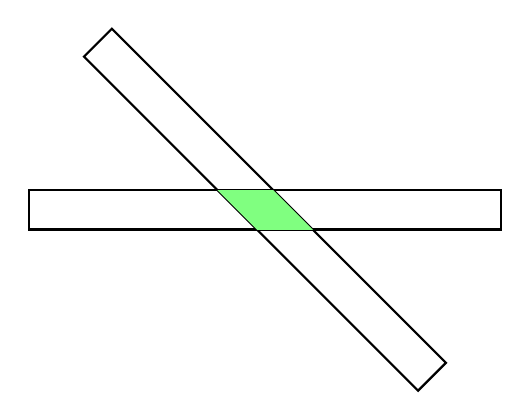
\begin{tikzpicture}
    % Draw first tube
    \draw[thick] (0,0) rectangle (6,0.5);
    % Draw second tube
    \draw[thick,rotate around={-45:(3,0.25)}] (0,0) rectangle (6,0.5);
    % Draw intersection area
    \begin{scope}
        \clip (0,0) rectangle (6,0.5);
        \fill[green!50,rotate around={-45:(3,0.25)}] (0,0) rectangle (6,0.5);
    \end{scope}
\end{tikzpicture}
\end{center}
We won't be able to show a direct equivalence since our methods accumulate logarithmic losses, but we can still achieve a pseudo-equivalence, which is quantified as follows: If $\delta=2^{-N}$, then
\begin{align*}
\Dec(\delta)\lesssim_\e \delta^{-\e}\BilinDec(\delta).
\end{align*}


We can also extend parabolic rescaling to the bilinear setting.

\begin{lem}\label{lem:bilinear parabolic}
Let $I$, $I' \in \Part(2^{-n})$ for some integer $n \geq 2$ such that $2^{-m}\leq\dist(I,I')<2^{-m+1}$ for some $m\leq n$.
For any $\delta \in (0,2^{-n})$ and any tuple of functions $(f_J)_{J \in \Part(I,\delta) \cup \Part(I',\delta})$ with $\supp \widehat{f_J} \subseteq \calU_{J}$ for all $J$, the following inequality holds:
\begin{equation} \label{eq:bilin_rescale}
\int_{\R^2} \abs{f_{I}}^{3} \abs{f_{I'}}^{3} \leq
\BilinDec(2^{m-2} \delta)^{6} \Bigl[ \sum_{J \in \Part(I,\delta)} \norm{f_J }_{6}^2 \Bigr]^{6/4}
\Bigl[ \sum_{J' \in \Part(I',\delta)} \norm{f_{J'} }_{6}^2 \Bigr]^{6/4}.
\end{equation}
\end{lem}

\begin{proof}
    Adapt the proof of \ref{lem:lin_rescale}
\end{proof}

\begin{lem}(Monotony of bilinear decoupling)
Given $0<\delta_L \leq \delta_S \leq 1$, $\BilinDec(\delta_L)\leq \BilinDec(\delta_S)$.
\end{lem}
\begin{proof}
Follows by Lemma (monotony decoupling).
\end{proof}

Let $M\in 2^\N$ and let $\mathcal{C}_M$ be the partition of $[0,1]$ into subintervals $\alpha$ with length $\frac{1}{M}$ so that $\abs{\mathcal{C}_M}=M$. We will write $\alpha\sim\alpha'$ if $\alpha$ and $\alpha'$ are neighbors of each other, and $\alpha\not\sim\alpha'$ otherwise. Notice that each $\alpha$ has at most $3$ neighbors (including itself). The following lemma provides us with a mechanism to deal with the superposition of waves and may be regarded as a model example of the so-called \textit{broad-narrow analysis}. (Add that the result is from Ciprian) 

\begin{lem}\label{bilinear linear elementary lemma}
There are constants $C$ (independent of $M$) and $C_M$ such that
\begin{align}\label{bilinear basic broad-narrow}
    \abs{\sum_{\alpha\in\mathcal{C}_M}z_\alpha}\leq C\max_{\alpha\in\mathcal{C}_M}\abs{z_\alpha}+C_{M}\max_{\alpha'\not\sim\alpha''}\abs{z_{\alpha'}z_{\alpha''}}^{1/2}
\end{align}
for any set of complex numbers $z_\alpha$ indexed by $\alpha\in\mathcal{C}_M$.
\end{lem}
\begin{proof}
Let $\alpha^*$ be such that $\abs{z_{\alpha^*}}=\max_{\alpha\in\mathcal{C}_M}\abs{z_\alpha}$. Define
\begin{align*}
    S_{big}\defeq \{\alpha\in\mathcal{C}_M \mid \abs{z_\alpha} \geq \frac{\abs{z_{\alpha^*}}}{K} \}
\end{align*}
to pick out the \textit{significant} terms on the left hand side of (\ref{bilinear basic broad-narrow}).

First suppose there exists $\alpha_0\in S_{big}$ such that $\alpha_0\not\sim\alpha^*$, then by definition of $S_{big}$ and the triangle inequality, we have
\begin{align*}
    \abs{z_{\alpha_0}z_{\alpha^*}}^{1/2}\geq\frac{\abs{z_{\alpha^*}}}{M^{1/2}}\geq\frac{\abs{\sum_{\alpha\in\mathcal{C}_M}z_\alpha}}{M^{3/2}},
\end{align*} 
which immediately implies that
\begin{align*}
    \quad\abs{\sum_{\alpha\in\mathcal{C}_M}z_\alpha}\leq M^{3/2}\max_{\alpha'\not\sim\alpha''}\abs{z_{\alpha'}z_{\alpha''}}^{1/2}.
\end{align*}
Hence we can choose $C_{M}=M^{3/2}$ on the right hand side of (\ref{bilinear basic broad-narrow}) to complete the proof.

Otherwise, every cube in $S_{big}$ must lie in the neighbor of $\alpha^*$, so we can dominate the left hand side of (\ref{bilinear basic broad-narrow}) using the triangle inequality:
\begin{align*}
    \abs{\sum_{\alpha\in\mathcal{C}_M}z_\alpha}&\leq\sum_{\alpha\sim\alpha^*}\abs{z_\alpha}+\sum_{\alpha\not\sim\alpha^*}\abs{z_\alpha}\\
    &\leq 3\abs{z_{\alpha^*}}+M\frac{\abs{z_{\alpha^*}}}{M}\\
    &=4\max_{\alpha\in\mathcal{C}_M}\abs{z_{\alpha}}.
\end{align*}
Therefore, we can choose $C=4$ on the right hand side of (\ref{bilinear basic broad-narrow}) to complete the proof.

Hence, in both cases (\ref{bilinear basic broad-narrow}) holds.
\end{proof}
\begin{thm}(Bilinear reduction)\label{thm:bilinear reduction} If $\delta=2^{-N}$, then for $n \leq N$
$$
\Dec(\delta)\leq C\Dec(2^{n}\delta) + C 2^{3n/2} \BilinDec(\delta)
$$
\end{thm}
\begin{proof}
    By using Lemma \ref{bilinear linear elementary lemma} with $K=2^k$, $\mathcal{C}_M = \Part(2^{-n})$, and $z_I = f_I(x)$, we have a pointwise inequality:
\begin{align*}
    \abs{F(x)} \leq 4\max_{I\in \Part(2^{-n})}\abs{f_I(x)} + 2^{3n/2} \max_{\substack{J_1,J_2\in\Part(2^{-n})\\ J_1 \not\sim J_2}} \abs{f_{J_1}(x)f_{J_2}(x)}^{1/2}.
\end{align*}

Taking the $L^6$-norm of both sides on $\R^2$, using the triangle inequality,  completing the sums, and finally using Minkowski's integral inequality, we get:
\begin{align*}
    \norm{F}_{L^6(\R^2)} 
    &\leq 
    4\norm{ \max_{J\in \Part(2^{-n})}\abs{f_J} }_{L^6(\R^2)} + 2^{3n/2} 
    \norm{ \max_{\substack{J_1,J_2\in\Part(2^{-n})\\ J_1 \not\sim J_2}} \abs{f_{J_1} f_{J_2}}^{1/2} }_{L^6(\R^2)}\\
    & \leq
    4\norm{\left(\sum_{J\in\Part(2^{-n})}\abs{f_J }^2\right)^{1/2}}_{L^6(\R^2)}
    +
    2^{3n/2} 
    \norm{ \left[\sum_{\substack{J_1,J_2\in\Part(2^{-n})\\ J_1 \not\sim J_2}} \left(\abs{f_{J_1} f_{J_2}}^{1/2}\right)^2 \right]^{1/2}}_{L^6(\R^2)} \\
    & \leq
    4 \left(\sum_{J\in\Part(2^{-n})}\norm{f_J}_{L^6(\R^2)}^2\right)^{1/2}
    +
    2^{3n/2} 
    \left(\sum_{\substack{J_1,J_2\in\Part(2^{-n})\\ J_1 \not\sim J_2}} \norm{\abs{f_{J_1}f_{J_2}}^{1/2}}_{L^6(\R^2)}^2 \right)^{1/2}.
\end{align*}

The first term is known as the narrow term, while the second is known as the broad term. 

Now, the strategy to bound both terms above is parabolic rescaling. For the first term, we can directly apply parabolic rescaling (Lemma \ref{lem:lin_rescale}),

\begin{align*}
\left(\sum_{J\in\Part(2^{-n})}\norm{f_J}_{L^p(\R^2)}^2\right)^{1/2}
    & \leq
    \Dec(2^{n}\delta) \left( \sum_{J\in\Part(2^{-n})} \sum_{J'\in\Part(J,\delta)} \norm{f_{J'}}_{L^6(\R^2)}^2 \right)^{1/2}\\
    & = \Dec(2^{n}\delta)\left(\sum_{J\in\Part(\delta)}\norm{f_{J'}}_{L^6(\R^2)}^2\right)^{1/2}.
\end{align*}
For the broad term, we observe that if $J_1$, $J_2 \in \Part(2^{-n})$ for some integer $n \geq 2$ and there is some $m\leq n$ such that $2^{-m}\leq\dist(I,I')<2^{-m+1}$, then by applying Lemma \ref{lem:bilinear parabolic} and using the monotonicity of the bilinear decoupling constant, we obtain,
\begin{align*}
    \norm{\abs{f_{J_1}f_{J_2}}^{1/2}}_{L^6(\R^2)}&\leq \BilinDec(2^{m-2}\delta)\left(\sum_{J\in\Part(J_1, \delta)}\norm{f_J}_{L^6(\R^2)}^2\sum_{J\in\Part(J_2, \delta)}\norm{f_J}_{L^6(\R^2)}^2\right)^{1/4}\\
    &\leq\BilinDec(2^{m-2}\delta)\left(\sum_{J\in\Part(\delta)}\norm{f_J}_{L^6(\R^2)}^2\right)^{1/2} \leq \BilinDec(\delta)\left(\sum_{J\in\Part(\delta)}\norm{f_J}_{L^6(\R^2)}^2\right)^{1/2}.
\end{align*}

Therefore, combining the estimates for both terms together, we obtain
\begin{align*}
    \norm{f}_{L^6(\R^2)}\leq \left(C\Dec(2^{n}\delta)+C2^{3n/2}2^{n}\BilinDec(\delta)\right)
    \left(\sum_{J\in\Part(\delta)}\norm{f_J}_{L^6(\R^2)}^2\right)^{1/2}
\end{align*}
which immediately implies that for any $n<N$:
\begin{align*}
    \Dec(\delta)\leq C\Dec(2^{n}\delta)+C_n\BilinDec(\delta).
\end{align*}
\end{proof}

\begin{cor}(Iteration) If $\delta=2^{-N}$, then
 \begin{align*}
    \Dec(\delta)\lesssim_\e \delta^{-\e}\BilinDec(\delta).
\end{align*} 
\end{cor}
\begin{proof}
Now we iterate the above inequality. The first few steps of the iteration looks like:
\begin{align*}
     \Dec(\delta)&\leq C\Dec(2^{-N+n})+C_n\BilinDec(\delta)\\
     &\leq C\left(C\Dec(2^{-N+2n}) + C_n\BilinDec(\delta)\right) + C_k\BilinDec(\delta)\\
     &\leq C^2\Dec(2^{-N+2n})+C_n(C+1)\BilinDec(\delta)
\end{align*}
If we repeat this $\frac{N}{n}$ times, then we would get
\begin{align*}
    \Dec(\delta)&\leq C^{N/n}\on\Dec(2^{-N+2\ceil{\frac{N}{n}}}n)+C_n(C^{N/n-1}+...+C+1)\BilinDec(\delta)\\
    &\lesssim C^{N/n}\left(1+C_n\BilinDec(\delta)\right)
\end{align*}
where we used the fact that $\Dec(2^{-N+2\ceil{\frac{N}{n}}}n)\sim \Dec(1/2) \lesssim1$ and computed the sum of the geometric series.


Finally, to conclude the argument we argue as follows. Fix any $\e>0$. If $N > \frac{\log_2C}{\e}+1$, then taking $k=\ceil{\frac{\log_2C}{\e}}<N$ yields
\begin{align*}
    \Dec(\delta)\lesssim 2^{N\e}\left(1+C_\e\BilinDec(\delta)\right)\lesssim_\e 2^{N\e}\left(1+\BilinDec(\delta)\right).
\end{align*}
On the other hand, if $N\leq\frac{\log_2C}{\e}+1$, then note that we always have the trivial estimate $\Dec(2^{-N})\leq 2^{N/2}$ by the Cauchy-Schwarz inequality, and therefore
\begin{align*}
    \Dec(\delta)\leq 2^{\frac{\log_2C}{2\e}+\frac{1}{2}}\lesssim_\e 1 \leq 2^{n\e}\left(1+\BilinDec(\delta)\right).
\end{align*}
Hence,
\begin{align*}
    \Dec(2^{-N})\lesssim_\e 2^{N\e}\BilinDec(2^{-N}).
\end{align*}
\end{proof}
Observation: we will be able to improve on the result to a log loss.
\newpage
\section{Asymmetric bilinear constant}
At this stage, our exposition diverges from the original Bourgain-Demeter argument [BD14]. We won't work with the bilinear constant itself, but with a similar bilinear object which was initially introduced by Li in []. 
(The full general form is highly inspired by the number-theoretic method known as efficient congruencing, developed by Wooley to prove the Vinogradov mean value theorem, see [Wooley15] or [Lilian Pierce].)

\begin{defn}\label{def>asymmetric bilinear}
For $a,b \in [0,1]$ and $\delta \in (0,1)$, the \emph{(asymmetric) bilinear decoupling constant} $\BilinDec_{a, b}(\delta)$ for the parabola is the smallest constant such that, for all pairs of intervals $I \in \Part(\delta^a)$, $I' \in \Part(\delta^b)$ with $\dist(I, I') \ge 1/4$ and all tuples of functions $(f_{J})_{J \in \Part(I,\delta) \cup \Part(I',\delta)}$ with $\supp \widehat{f_{J}} \subseteq \calU_{J}$ for all $J$, the following inequality holds:

\begin{equation}
\label{eq:asymetric constant}
 \int_{\R^2} \abs{f_{I}}^{2}  \abs{f_{I'}}^{4}
\leq \BilinDec_{a, b}(\delta)^{6}\Bigl( \sum_{J \in \Part(I,\delta)} \norm{f_J }_{6}^2 \Bigr) \Bigl( \sum_{J' \in \Part(I',\delta)} \norm{f_{J'} }_{6}^2 \Bigr)^{2}.
\end{equation}
\end{defn}
By using Hölder's inequality we have $\BilinDec_{a, b}\lesssim \delta^{-1/2}$.

The $\BilinDec_{a, b}$ encodes the cost to decouple two intervals of size $\delta^ a$ and $\delta^b$ respectively into intervals of size $\delta$. 
Informally, by considering \(a = b\) and taking \(a \approx 1\), then \(\delta^a \approx C_{1}\delta\) for some \(C_{1} > 0\), so the cost to decouple both \(I\) and \(I'\) into intervals of size \(\delta\) will be a constant \(C_{2}\). Thus, as in the case of almost multiplicity, it is a desirable property to control \(\BilinDec_{a, b}\) by some decoupling constant at a larger scale.
\newline
In the case of the parabola we can in fact prove the following:

\begin{lem}[White lie 1] \label{lem:b}
Let $\delta \in (0,1)$ and $(f_K)_{K \in \Part(\delta)}$ be a tuple of functions so that $\supp \widehat{f_K} \subset \calU_K$ for every $K$.
If $0 \leq a \leq 2b$, then, for any pair of frequency intervals $I \in \Part(\delta^a)$, $I' \in \Part(\delta^b)$ with $\dist(I,I') \geq 1/4$, we have
\begin{equation}\label{eq:fiber-dec}
    \int_{\R^2}  \abs{f_{I}}^{2}\abs{f_{I'}}^{4} \lesssim \sum_{J\in \Part(I,\delta^{2b})}  \int_{\R^2} \abs{f_{J}}^{p_{l}} \abs{f_{I'}}^{4} .
\end{equation}
\end{lem}
By the definition of asymmetric bilinear decoupling constants this results immediately implies the following:
\begin{thm}\label{thm: key step}
For any $0 \leq a \leq 2b$ and $\delta \in (0,1)$, we have
\[
\BilinDec_{a,b}(\delta)
\lesssim
\BilinDec_{2b, b}(\delta).
\]
\end{thm}

This theorem is a manifestation the the phenomenon described above, we can controller the asymmetric billinear constant, $\BilinDec_{a,b}$, by a decoupling constant at a bigger scale, $\BilinDec_{2b,b}$.\\

To justify the sufficient of only studying the asymetric bilinear constant the following results justifies that:
\begin{lem}
For $a, b \in[0,1]$ and $\delta \in(0,1 / 4)$, we have
\begin{equation*}
\mathcal{B}(\delta) \lesssim \delta^{-a/3 } \delta^{-2b/3} \mathcal{B}_{a, b}(\delta) 
\end{equation*}
\end{lem}

\begin{proof}
     Let $I, I^{\prime} \in \mathcal{P}(1 / 4)$ with $\operatorname{dist}\left(I, I^{\prime}\right) \geqslant 1 / 4$. Let $\left(f_{K}\right)_{K \in \mathcal{P}(I, \delta) \cup \mathcal{P}\left(I^{\prime}, \delta\right)}$ be a tuple of functions with $\operatorname{supp} \widehat{f_{K}} \subseteq \mathcal{U}_{K}$ for all $K$. By Hölder's inequality, we have

\begin{equation*}
\int_{\mathbb{R}^{2}}\left|f_{I}\right|^{3}\left|f_{I^{\prime}}\right|^{3} \leqslant
\left(\int_{\mathbb{R}^{2}}\left|f_{I}\right|^{2}\left|f_{I^{\prime}}\right|^{4}\right)^{1 / 2}\left(\int_{\mathbb{R}^{2}}\left|f_{I}\right|^{4}\left|f_{I^{\prime}}\right|^{2}\right)^{1 / 2} 
\end{equation*}
It suffices to estimate the first term. Again by Hölder's inequality 
\begin{equation}
\int_{\mathbb{R}^{2}}\left|f_{I}\right|^{2}\left|f_{I^{\prime}}\right|^{4}\leqslant \int_{\mathbb{R}^{2}}\left(\sum_{J \in \mathcal{P}\left(I, \delta^{a}\right)}\left|f_{J}\right|\right)^{2}\left(\sum_{J^{\prime} \in \mathcal{P}\left(I^{\prime}, \delta^{b}\right)}\left|f_{J^{\prime}}\right|\right)^{4}
\end{equation}
\begin{equation}
    \leqslant \left|\mathcal{P}\left(I, \delta^{a}\right)\right|^{1}\left|\mathcal{P}\left(I^{\prime}, \delta^{b}\right)\right|^{3} \sum_{J \in \mathcal{P}\left(I, \delta^{a}\right)} \sum_{J^{\prime} \in \mathcal{P}\left(I^{\prime}, \delta^{b}\right)} \int_{\mathbb{R}^{2}}\left|f_{J}\right|^{2}\left|f_{J^{\prime}}\right|^{4}
\end{equation}
By Definition \ref{def>asymmetric bilinear},
\begin{equation}
\int_{\mathbb{R}^{2}}\left|f_{I}\right|^{2}\left|f_{I^{\prime}}\right|^{4} \lesssim \delta^{-a} \delta^{-3b} \mathcal{B}_{a, b}(\delta)^{6}\left[\ell_{K \in \mathcal{P}(I, \delta)}^{2}\left\|f_{K}\right\|_{6}\right]^{2}\left[\ell_{K^{\prime} \in \mathcal{P}\left(I^{\prime}, \delta\right)}^{2}\left\|f_{K^{\prime}}\right\|_{6}\right]^{4}
\end{equation}
\end{proof}

In this section, we won’t provide a rigorous proof for Lemma \ref{lem:b}, which is why we refer to it as a "white lie." For a fully rigorous approach, one would need to formalize our use of the uncertainty principle, see [zane parabola]. However, to focus on presenting the main ideas, delving into this formalization could lead to getting lost in the details.

In the remaining part of the section, we'll show two approaches to achieving such a result. The first approach, in the style of BDG, relying on wave packet decomposition, and the second will be a sketch of the proof by [ShortProof] in the parabola case. We defer these details to the sources, [zane harmonic QP] [video series].
\newline
Common to two approaches, we need a form of decoupling, commonly known as $local$ $L^2$-$orthogonality$.
\begin{lem}[White lie 2]\label{white lie2}
    For $l=1,2$, for $\delta \in (0,1)$, and $B$ be a ball of of a cube in $\R^l$ of radius or side length $\delta^{-l}$. Then,
    \begin{equation}\label{eq:local decoupling}
    || f||_{L^{2}(B)}^{2} \lesssim \sum_{J\in\Part(\delta)} || f_{J}||_{L^{2}(B)} ^{2}
    \end{equation}
\end{lem}
This lemma isn't fully rigorous, since the RHS of \ref{eq:local decoupling} should have a weight instead of a sharp cut-off. (Give a sketch)




\subsection{Wave packet approach}\label{subsection:Wave packet approach}
Take $I,I'  \in \Part(\delta^b)$, with $\dist(I, I') \ge 1/4$. Explain dual box. By the uncertainly principle, $|f_{I}|$ will be essentially constant on translates of the dual box $\freqU_{I}$. Denote as $\mathcal{B}(I)$ the tilling of $\R^2$ by translated copies of $\freqU_{I}$, then it at least morally the following identity is true


\begin{equation}\label{eq: heuristic wave packet}
    |f_{I}| \sim \sum_{T // \, \freqU_{I}} c_{T} 1_{T}.
\end{equation}

To turn this into a true identity we would need the full wave packet decomposition (appendix). 

We can use this decomposition to compute a localize version of the LHS of \ref{eq:BilinDec}. \ref{eq:BilinDec}

\begin{equation}\label{eq:part1 packet}
    \fint_{B(0,\delta^{-2b})} \abs{f_{I}}^{2}  \abs{f_{I'}}^{4} \leq  \sum_{} c_{T}^{2}c_{T^{\prime}}^{4} \frac{|T\cap T^{\prime} |}{|B(0,\delta^{-2b})|} =  \sum_{} c_{T}^{2}c_{T^{\prime}}^{4} \delta ^{2b},
\end{equation}
where in the equality we used the fact that since the intervals are unit separated $T$ and $T'$ will intersected almost orthogonally, so $|T\cap T'|\sim \delta^{-2b}$.

Observe that,
\begin{equation}\label{eq:part2 packet}
     \sum_{} c_{T}^{2}c_{T^{\prime}}^{4} \delta ^{2b} = \sum_{}  c_{T}^{2} \frac{|T|}{|B(0,\delta^{-2b})|} \sum_{}c_{T^{\prime}}^{4} \frac{|T^{\prime}|}{|B(0,\delta^{-2b})|} = \left(\fint_{B(0,\delta^{-2b})}\abs{f_{I}}^{2} \right) \left(\fint_{B(0,\delta^{-2b})}\abs{f_{I^{\prime}}}^{4}   \right).
\end{equation}
Combining \ref{eq:part1 packet} and \ref{eq:part2 packet} yields,

\begin{equation}\label{eq: wave packet local}
\fint_{B(0,\delta^{-2b})} \abs{f_{I}}^{2}  \abs{f_{I'}}^{4}
\leq \left(\fint_{B(0,\delta^{-2b})}\abs{f_{I}}^{2} \right) \left(\fint_{B(0,\delta^{-2b})}\abs{f_{I^{\prime}}}^{4}   \right)
\end{equation}


Now we can apply a local $L^{2}$-orthogonality, i.e, 

\begin{equation}
    \fint_{B(0,\delta^{-2b})}\abs{f_{I}}^{2} \lesssim  \sum_{J\in\Part(I,\delta^{2b})} \fint_{B(0,\delta^{-2b})} |f_{J}|^2.
\end{equation}
By the uncertainly principle, since $|J| = \delta^{2b}$, then $|f_{J}|$ is essentially constant on the dual tube $\mathcal{F}_{J}$, which has dimensions $\delta^{-2b} \times \delta^{-4b}$. Consequently, $B(0,\delta^{-2b})$ is contained in the dual tube, so combining this with \ref{eq: wave packet local} yields

\begin{equation}
    \fint_{B(0,\delta^{-2b})} \abs{f_{I}}^{2}  \abs{f_{I'}}^{4} \lesssim \sum_{J\in\Part(I,\delta^{2b})} \fint_{B(0,\delta^{-2b})} |f_{J}|^2 |f_{I^{\prime}}|^4.
\end{equation}
By introducing a modulation on $f$ we can extend this results to,
\begin{equation}
    \fint_{B} \abs{f_{I}}^{2}  \abs{f_{I'}}^{4} \lesssim \sum_{J\in\Part(I,\delta^{2b})} \fint_{B} |f_{J}|^2 |f_{I^{\prime}}|^4.
\end{equation}
where $B$ is a ball of arbitrary center and radius $\delta^{-2b}$. Since we can tile the plane by a countable family of finite-overlapping balls we get Lemma \ref{lem:b}.


\subsection{Averaging approach/lower dimensional approach}\label{subsection:Averaging approach}
Based on [Lecture 22, Hickman] we can summarized the second approach with the following  
\begin{figure}[h!]
    \centering
    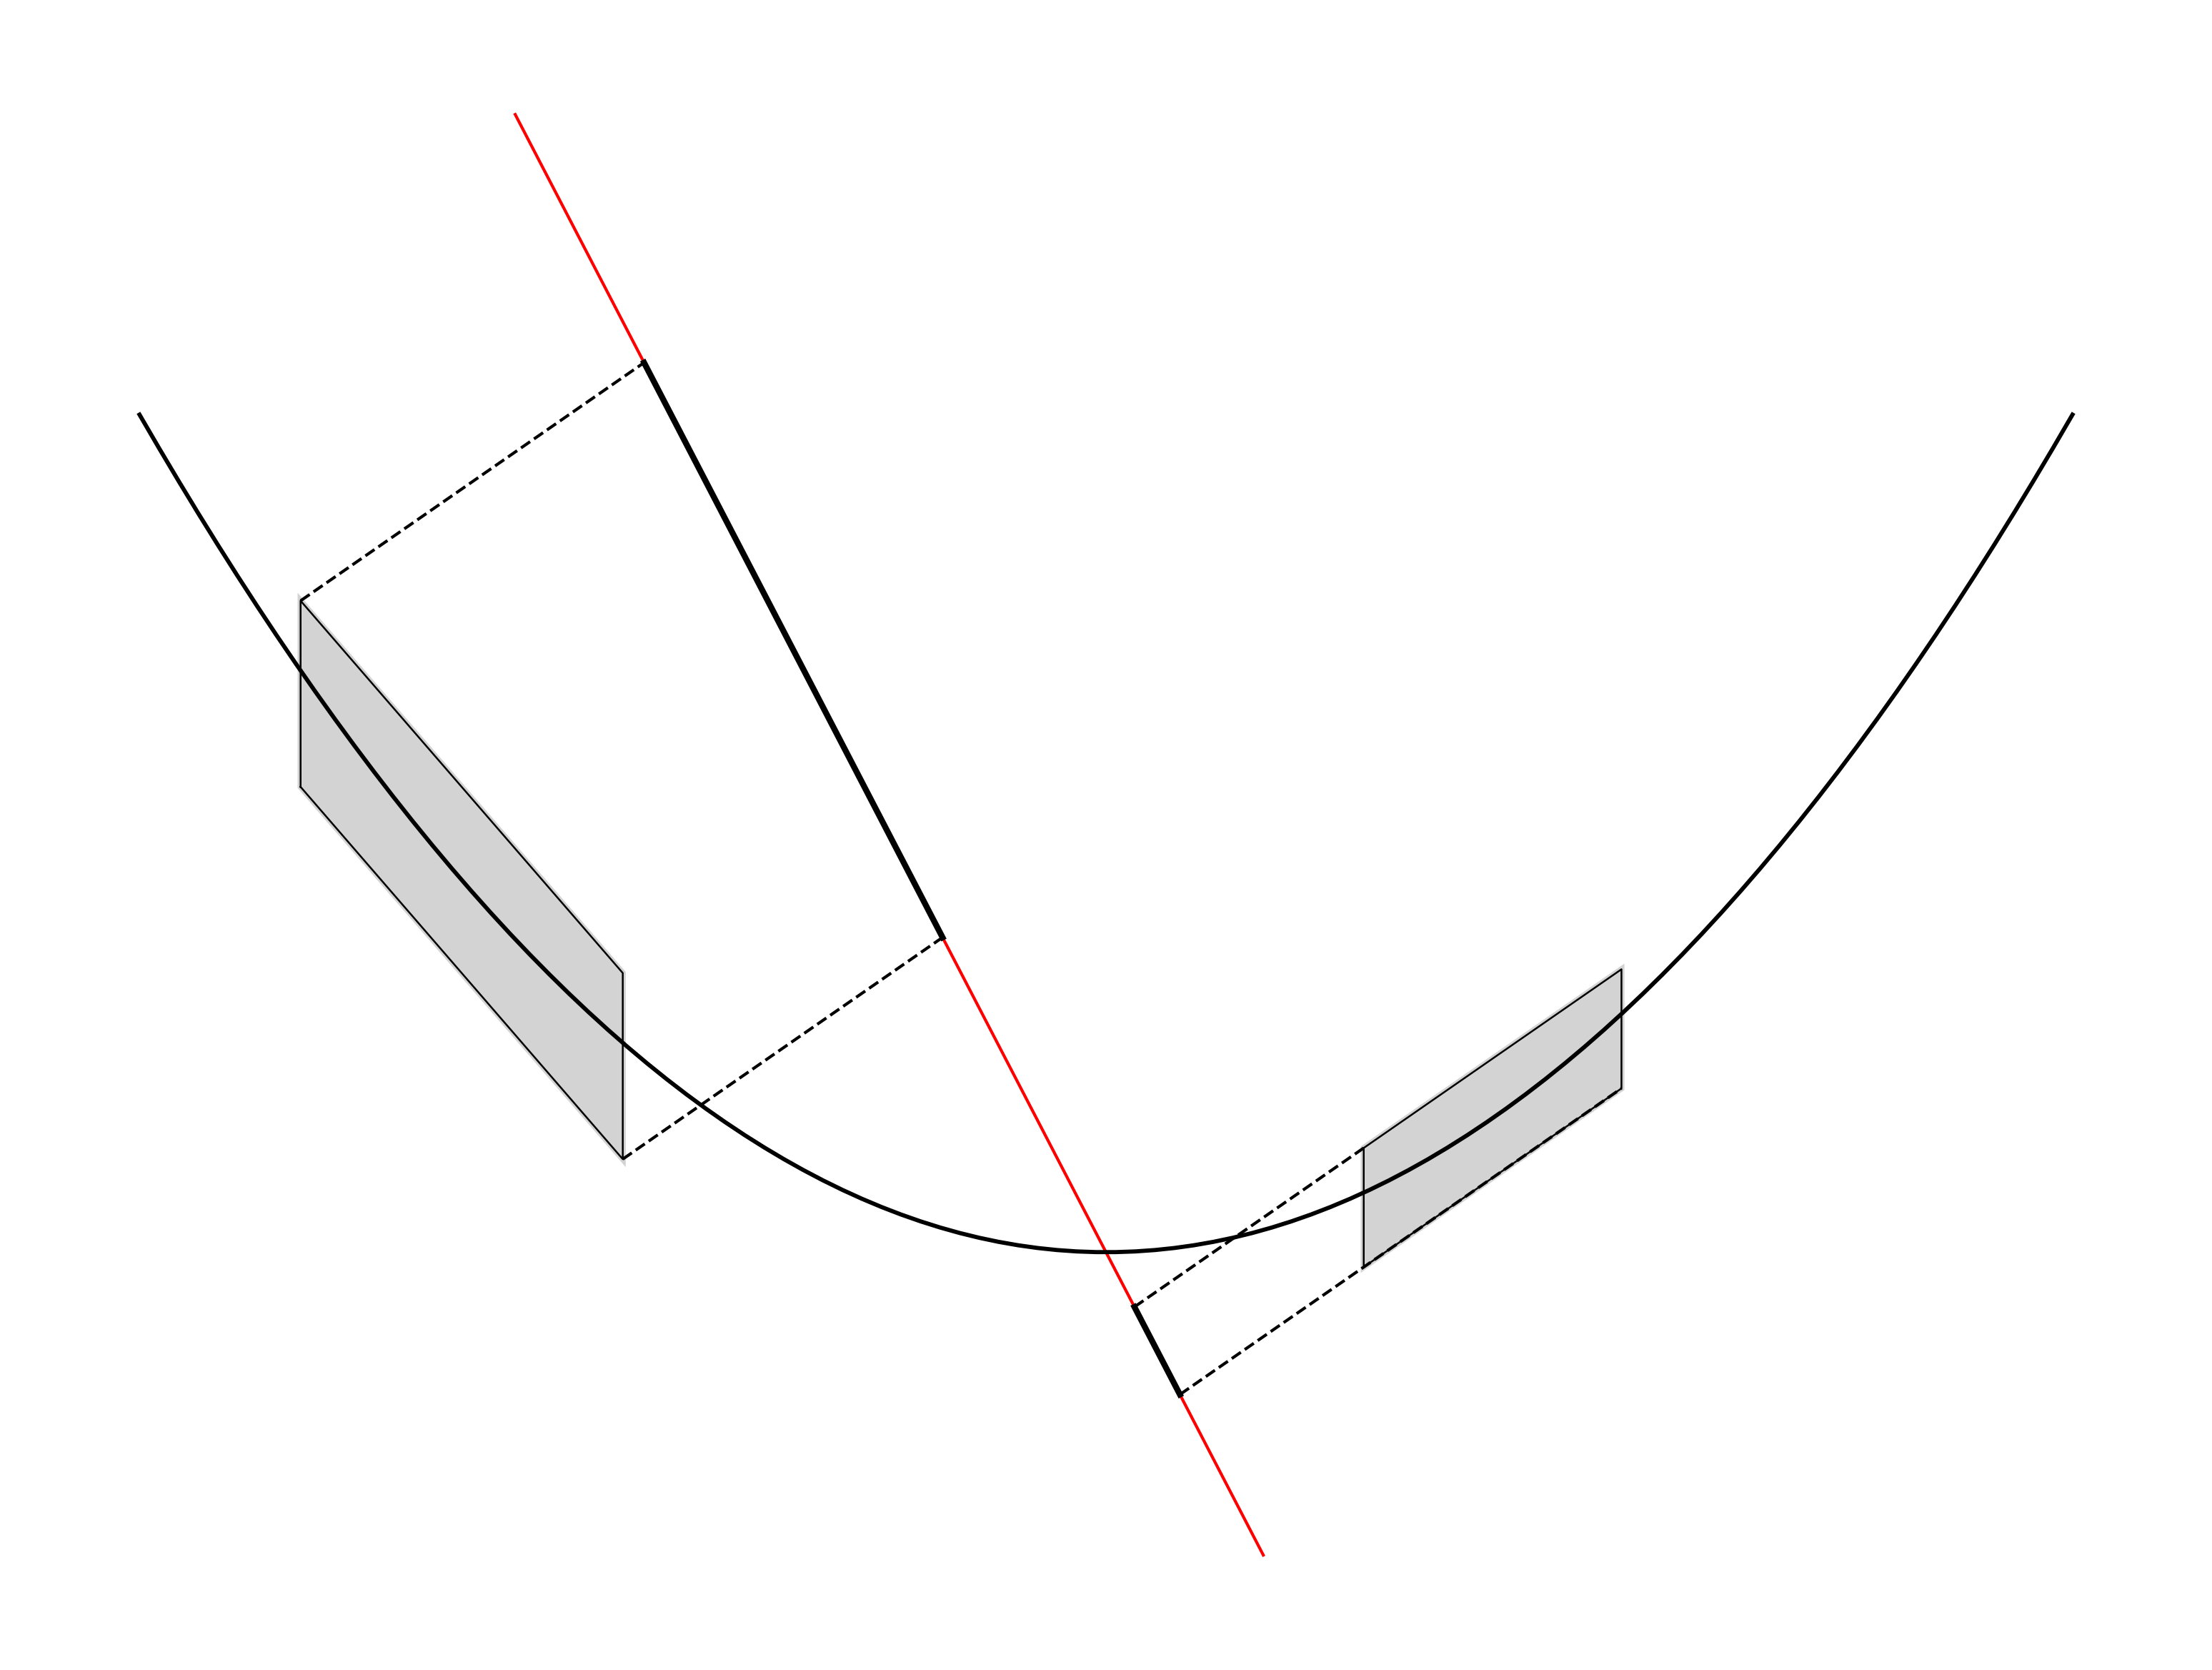
\includegraphics[scale=0.6]{Pics/Proj1.png}
    \caption{Projections }
    \label{fig:projections}
\end{figure}


Consider $I\in \Part(I,\delta^{a})$ and $I^{\prime}\in \Part(I^{\prime},\delta^{b})$, such that $dist(I,I')\geq 1/4$ $\hat{f_{I}}$, $\hat{f_{I^{\prime}}}$ are supported on $\calU_{I}$ and $\calU_{I^{\prime}}$, respectively. Let $\nu:[-1,1]\xrightarrow{}$

For $c_{I^{\prime}}$ define $H = Span\{\nu(c_{I^{\prime}})\}$ to be the subspace of $\R^2$ spanned by $\nu(c_{I^{\prime}})$, see red line in \ref{fig:projections}.

Let $\text{Proj}_{\,H}: \R^{d}\longrightarrow H$, then we have the following geometric consequences,

$$diam(\text{Proj}_{\,H}(\calU_{I^{\prime}}))\lesssim \delta^{2b},$$

in particular we see that $\calU_{I^{\prime}}$ is projects onto a line segment of length $\delta^{2b}$ which corresponds to the shorts side of $\calU_{I^{\prime}}$.

On another hand the unit separation of the intervals translates to a form of tranversality between $\calU_{I}$ and $\calU_{I^{\prime}}$, i.e,
$$
diam(\text{Proj}_{\,H}(\calU_{I}))\sim \delta^{a}
$$
in particular $\calU_{I}$ is projected onto a interval of length $\delta^a$, which corresponds to the long side of $\calU_{I}$.

Now we want to subdivide the interval $I$ into intervals of a smaller scale and then consider what happens to the frequency boxes under this projection map. To make this more precise let $0\leq \eta \leq \delta^ a$, then 

\begin{equation}\label{eq:sub projections}
\{\text{Proj}_{\,H}(\calU_{K}):\, K\in \Part(I,\eta)\}
\end{equation}
is a family of finite-overlapping intervals of length $\sim \eta$.
\begin{figure}[h!]
    \centering
    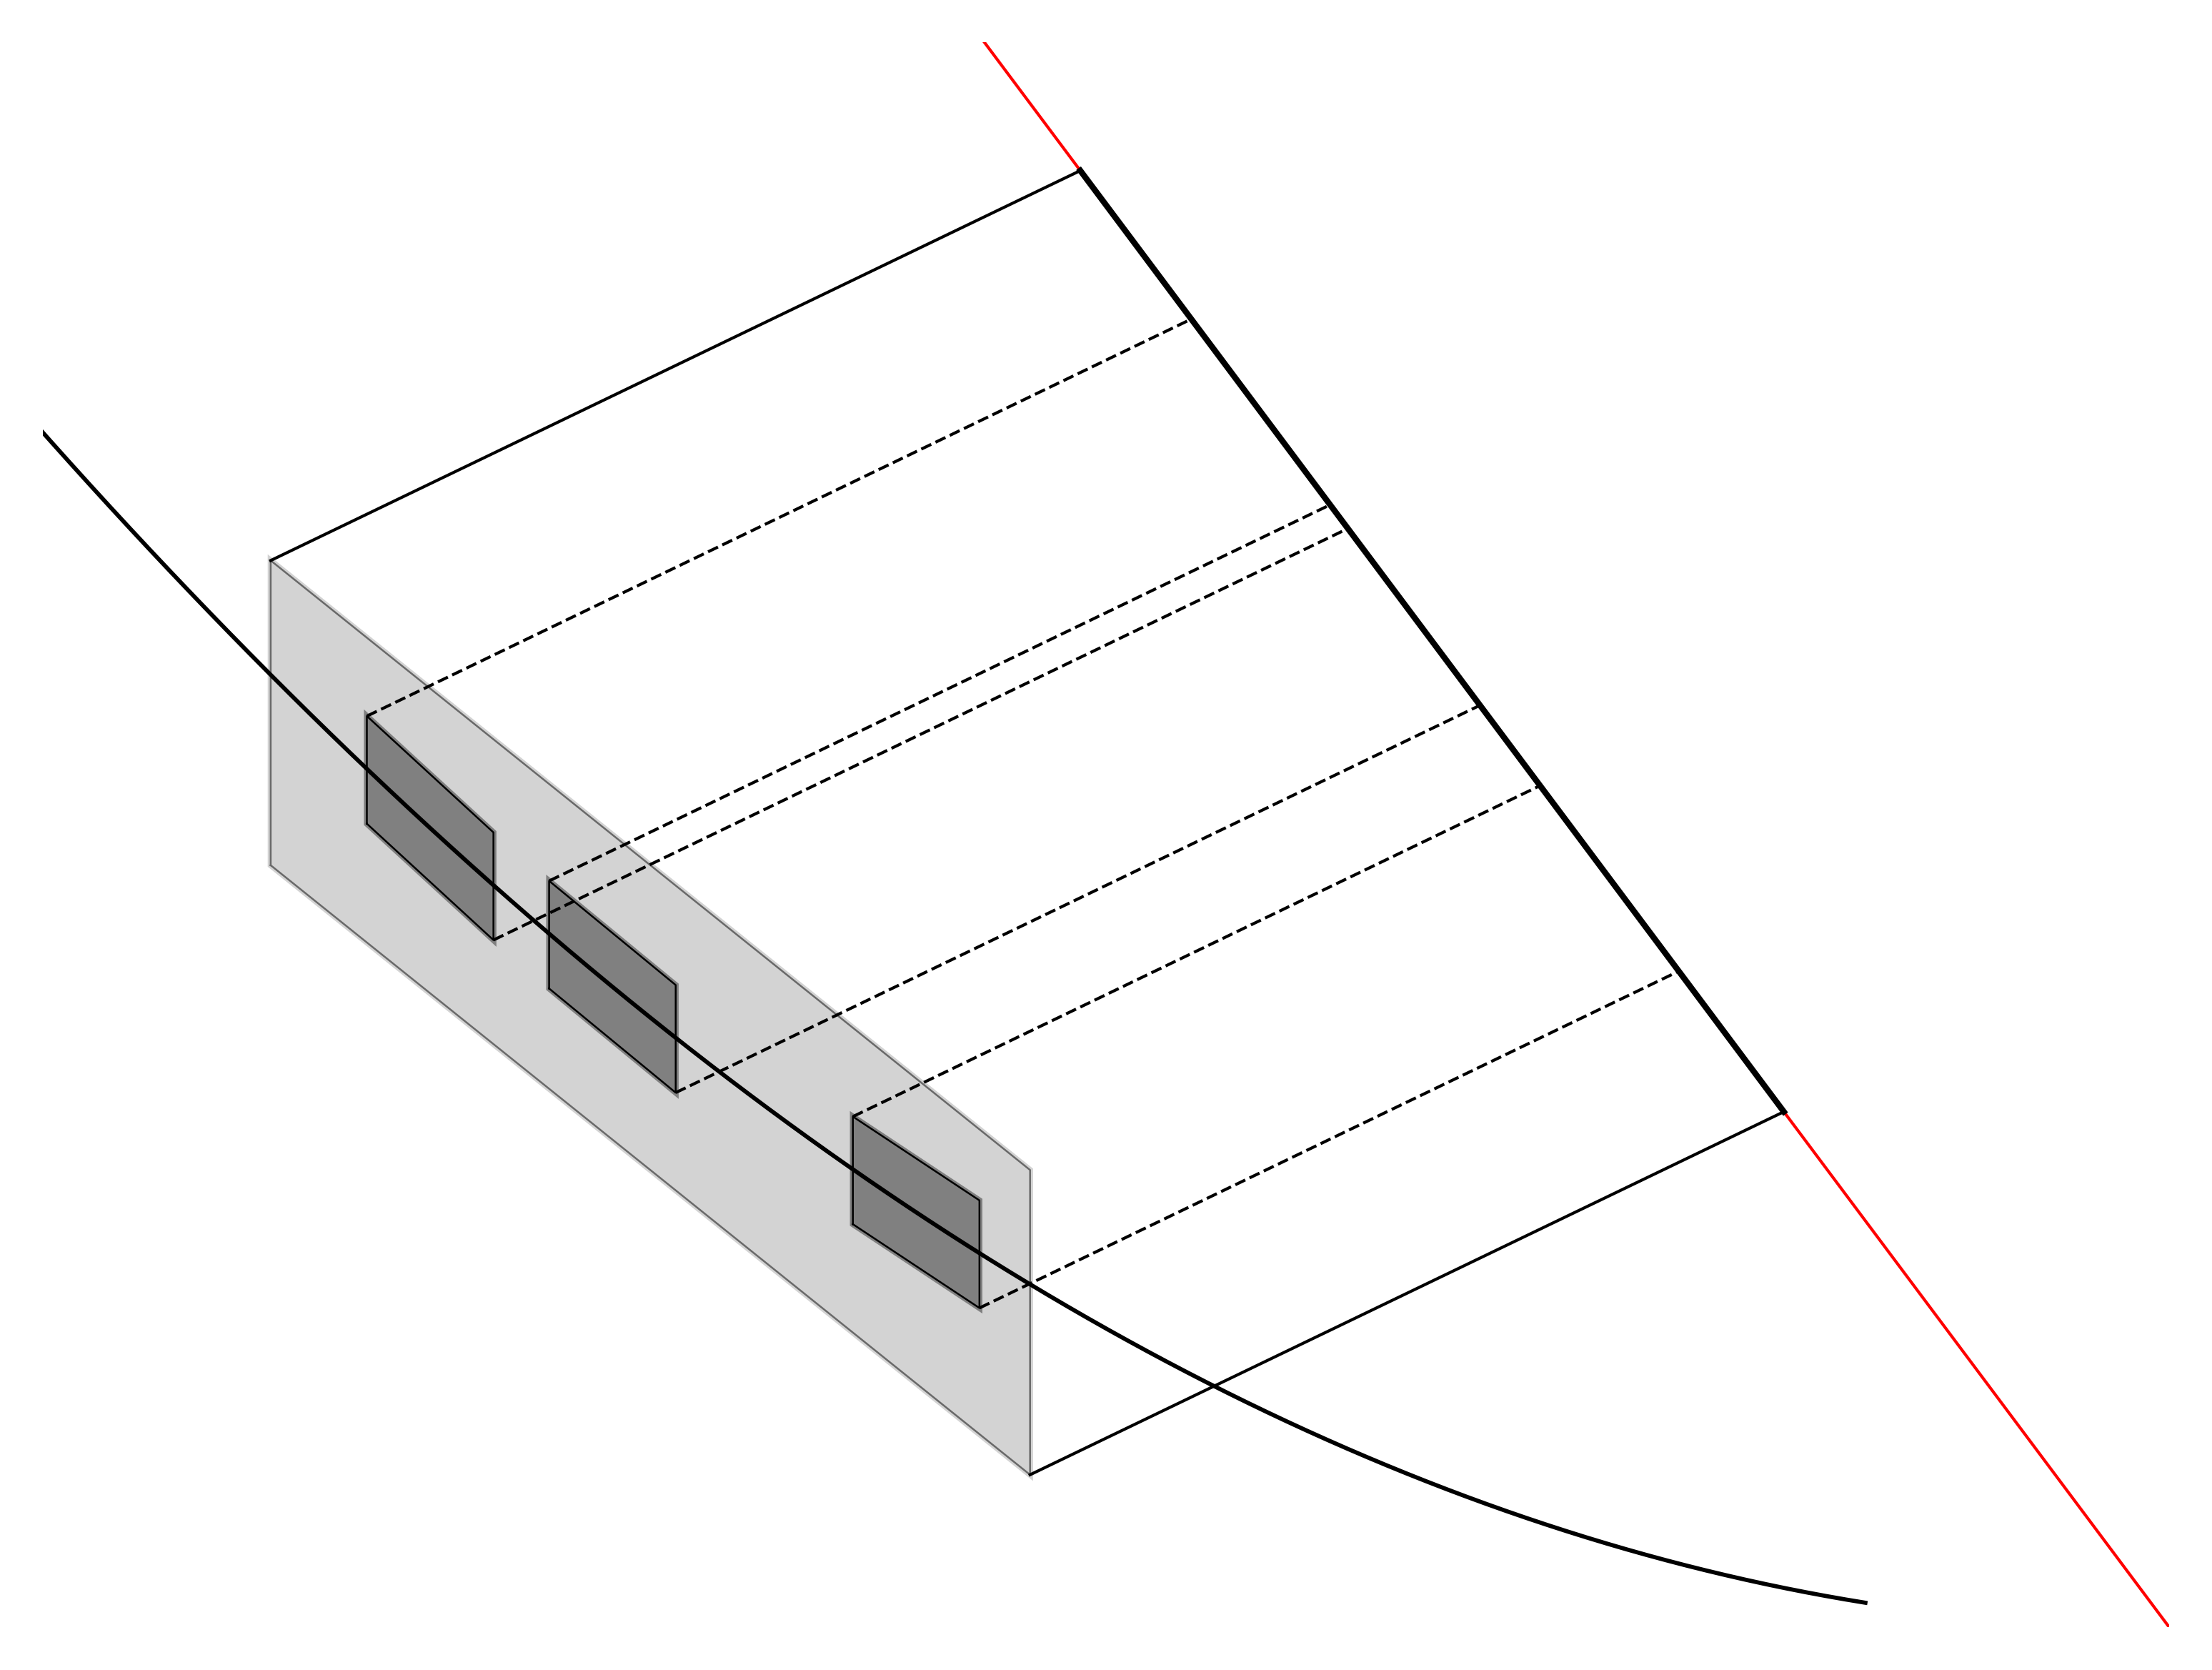
\includegraphics[scale=0.6]{Pics/Proj2.png}
    \caption{Projections}
    \label{fig:projections_overlap}
\end{figure}


To convert all this geometric facts into analytical form, one needs the following auxiliary lemma.
\begin{lem}\label{lem:fourier projecton} 
    Let $f\in \mathcal{S}(\R^d)$ and write $x=(x^{\prime},x^{\prime\prime})\in \R^{k} \times \R^{d-k}$. For each $x^{\prime\prime}$ consider the slice $f_{x^{\prime\prime}}: \R^{k}\longrightarrow \C$ define as $f_{x^{\prime\prime}}(x^{\prime}):=f(x^{\prime},x^{\prime\prime})$,
    then
    $$
    \supp(\, \widehat{f_{x^{\prime\prime}}}) \,\subset \text{Proj}_{\,\R^{k} }(\supp \hat{f})
    $$
    where $\text{Proj}_{\,\R^{k}}: \R^{d}\longrightarrow \R^{k}$; $(\xi^{\prime},\xi^{\prime\prime})\xrightarrow{}\xi^{\prime}$ denotes the orthogonal projection.
\end{lem}
\begin{proof}
    By Fubini's Theorem we can argue,
    \begin{equation}\label{eq:fourier slice}
        \hat{f}(\xi) = \int_{\R^d} f(x^{\prime},x^{\prime\prime}) e(x^{\prime }\cdot \xi^{\prime})e(x^{\prime\prime}\cdot \xi^{\prime})\, dx^{\prime}dx^{\prime\prime} = \int_{\R^{d-k}} (\widehat{f_{x^{\prime\prime}}})(\xi^{\prime})e(x^{\prime\prime}\cdot \xi^{\prime})dx^{\prime\prime} = \mathcal{F}_{x^{\prime\prime}}\left[ \widehat{f_{x^{\prime\prime}}}(\xi^{\prime})\right]
    \end{equation}
    Where $\mathcal{F}_{x^{\prime\prime}} $, denotes the Fourier transform in the $x^{\prime\prime}$ variable.\\
    
    If \(\xi' \not\in \text{Proj}_{\,\R^{k}}(\supp \hat{f})\), then for any \(\xi'' \in \R^{d-k}\), we have \((\xi', \xi'') \not\in \supp \hat{f}\). Therefore, by \eqref{eq:fourier slice}, \(\mathcal{F}_{x''}\left[\widehat{f_{x''}}(\xi')\right] = 0\). Since the Fourier transform is injective, this implies \(\widehat{f_{x''}}(\xi') = 0\). Consequently, \(\xi' \not\in \supp(\widehat{f_{x''}})\).

\end{proof}

From this we see that if we have some function $f_{J}$ in $\mathbb{R}^{2}$ with Fourier support in $\cal{U}_{J}$, then the restriction, $\left.f_{J}\right|_{H}$, of $f_{J}$ to some $1$-dimensional manifold $H$ has its Fourier support contained the projection of $\cal{U}_{J}$ onto $H$.

\begin{lem}
    Let $d\geq 1$ and  $H$ a $k$-dimension linear subspace of $\R^d$. Then by choosing coordinates as in Lemma \ref{lem:fourier projecton},

$$
\int_{\R^2}f =\int_{z\in \R^d}\fint_{B_{H}(x,r)} f
$$
where $B_{H}(x,r)$ is a ball of center $x$ and radius $r>0$, contained in $H$.
\end{lem}
\begin{proof}
    Applying Fubini's Theorem gives

$$
\int_{x\in \R^d}\fint_{B_{H}(x,r)} f = \int_{x\in \R^d} \fint_{B_{\R^2}(0,r)} f(x' + y,x'') \,dy = \fint_{B_{\R^2}}\int_{x\in \R^d} f(x' + y,x'') \,dx\,dy = \int_{x\in \R^d} f.
$$
\end{proof}
Now, we apply this averaging argument to our particular case:
\begin{equation}
\int_{\R^2} \abs{f_{I}}^{2} \abs{f_{I'}}^{4} \,
= \int_{\R^2} \fint_{B_{H}(x,\delta^{-2b})} \abs{f_{I}}^{2} \abs{f_{I'}}^{4} \,.
\end{equation}
By orthogonality, we can argue that $B_{H}(0,\delta^{-2b}) \subseteq \freqU_{I}$ and so, $|f_I|$ is essentially constant on $B_{H}(0,\delta^{-2b})$. Now we apply $L^2$ orthogonality to $\left.f_{I}\right|_{H}$ with radius $\delta^{-2b}$:
$$
\int_{\R^2}\abs{f_{I'}}^{4} \fint_{B_{H}(x,\delta^{-2b})} \abs{f_{I}}^{2}  \, dy \, dx \leq \int_{\R^2}\abs{f_{I'}}^{4} \sum_{J\in\Part(I,\delta^{2b})} || f_{J}||_{L^{2}(B_{H}(x,\delta^{-2b}))} ^{2} = \sum_{J\in\Part(I,\delta^{2b})}\int_{\R^2}|f_{J}|^2\abs{f_{I'}}^{4}.
$$
Observe that the chosen radius is maximal.



\section{Bootstrap}\label{section:bootstrap}
In this section we prove Theorem \ref{thm:main} by using Lemma \ref{thm: key step}.

\begin{lem}[Swap] \label{lem:Hölder}
    If $a, b \in (0,1)$ and $\delta \in (0,1)$, then
\begin{equation}\label{eq:Hölder}
\BilinDec_{a,b}(\delta)
\leq
\BilinDec_{b,a}(\delta)^{\frac{1}{2}} \Dec(\delta^{1-b})^{\frac{1}{2}}.
\end{equation}
\end{lem}
\begin{proof}
By Hölder's inequality,
    \begin{equation}
    \int_{\R^2} |f_I|^2|f_{I^{\prime}}|^4\, dx \leq \left(\int_{\R^2} |f_{I^{\prime}}|^2|f_I|^4\, dx \right)^{\frac{1}{2}}\left(\int_{\R^2}|f_{I}^{\prime}|^6 \, dx \right)^{\frac{1}{2}}.
    \end{equation}

The results follows from the definition of $\BilinDec_{a,b}$ and parabolic rescaling.
\end{proof}

\begin{lem}[Iteration]\label{lem:iteration}
For $b\in [0,1]$ and $b\leq \frac{1}{4}$ we have,
$$
\BilinDec_{2b,b}(\delta) \lesssim (\BilinDec_{4b,2b}(\delta)) ^{\frac{1}{2}}(\Dec(\delta^{1-b})) ^{\frac{1}{2}}
$$  
\end{lem}
\begin{proof}
    Apply Theorem \ref{thm: key step} followed by \ref{lem:Hölder}.
\end{proof}


\begin{proof}[Sketch of Theorem \ref{thm:main}]
Let $\eta$ be the infimum of all $\epsilon$ for which the decoupling inequality \eqref{eq:main} holds.

Define $A_1(b)$ to the the smallest exponent such that 
$$
\BilinDec_{2b,b}(\delta) \lesssim \delta^{-A}
$$
and $A_0(b)$ be the smallest exponent such that

$$
\Dec(\delta^{1-b}) \lesssim \delta ^{-A}.
$$
A direct calculation gives $A_0(b)=\eta(1-b)$.

By applying this definitions to Lemma \ref{lem:iteration},

$$
\BilinDec_{2b,b}(\delta) \lesssim \left[ \delta^{-A_{1}(2b)}\right]^{\frac{1}{2}}\left[ \delta^{-\eta(1-b)}\right]^{\frac{1}{2}}
$$
which can be simplified to 
\begin{equation}\label{eq:iter proof}
A_1(b) \leq A_{1}(2b) + \eta(1-b).
\end{equation}


We extract the information on the asymptotic behaviour of bilinear decoupling exponents $A_{l}(b)$ from the functional inequality \eqref{eq:iter proof} by introducing the quantities
$$
A_{l} := \liminf_{b\to 0} \frac{\eta - A_{l}(b)}{b} \in \R \cup \{\pm\infty\}.
$$

which yields
$$
A_1 \geq A_1 + \frac{1}{2} \eta.
$$

By assuming that $A_1$ is a finite this is equivalent to the claim. (This happens because there is an equivalence between linear and bilinear decoupling)


\end{proof}











































\chapter{Moment curve}
We need a small intro explaining the purpose of this chapter, like the main goal is to prove the Vinagradov mean value theorem. 
For that we prove the more general result about decoupling and then use it in the context of exponential sums.\\

Introduce the definition. Maybe motivate why this partion is natural in the case of curves. It has to obey nicely an affine rescaling (Guth notes). \\

Move onto the the bilinear reduction. Calculations for the change of variables.  Whitney (tenho de fazer boneco). \\

Introduce billinear assymetric, mention that the BDG object is more complicated. Talk about the tranversality is captured by the assymetric constantes.\\

Change the proof of lower degree decoupling (call it Pranik-Seeger iteration because this is how we extend the result to the circle for instance). Show how to prove the dilation.\\ 

Key lemma, show to get the C. Use the picture to explain. Use the reduction, where one box uses the center. Refer back to the averaging result showed in parabola. (Invoke appendix lemmas). 

Do the final steps for the iteration.\\

(one needs the linear algebra result).
\newpage
\section{Intro stuff - geometry and definitions}
To generalize the work done in Chapter 2, we need to establish which neighborhood of the curve we are choosing and how to partition it in \(\mathbb{R}^k\). For curves, the appropriate scale to consider is \(\delta^k\). This choice essentially arises from the need to obtain the correct scale when reframing the problem under a change of coordinates [Guth, Lecture18].


Let $\Gamma:[0,1] \rightarrow \mathbb{R}^{k}$ be the moment curve in $\mathbb{R}^{k}$, parametrized by 
$$
\Gamma(\xi):=\left(\xi, \xi^{2}, \ldots, \xi^{k}\right).
$$
Let $\theta$ be a $\delta^k$-arc of the moment curve, i.e, is $\Gamma([a,a+\delta^k])$ for some $a$. Then by Taylor expansion, 


$$\Gamma(t)=\Gamma\left(c_a\right)+\Gamma^{\prime}\left(c_a\right) \Delta t+\frac{1}{2} \Gamma^{\prime \prime}\left(c_a\right) \Delta t^{2}+\cdots+\frac{1}{k!} \Gamma^{(k)}\left(c_a\right) \Delta t^{k}$$. 

Observing that  $\Delta t^j$ as size proportional to $\delta^j$ and that $\Gamma^{\prime}\left(c_a\right), \Gamma^{\prime \prime}\left(c_a\right), \cdots, \Gamma^{(k)}\left(c_a\right)$ are linear independent the smallest box that can contain $\theta $ has dimensions $\delta \times \delta^2\times \cdots \delta^k$. 

For $\delta \in(0,1)$, let $\mathcal{P}(\delta)$ denote the partition of the interval $[0,1]$ into dyadic intervals with length $2^{-\left\lceil\log _{2} \delta^{-1}\right\rceil}$. For a dyadic interval $J$, let $\mathcal{U}_{J}$ be the parallelepiped of dimensions $|J|^{1} \times|J|^{2} \times \cdots \times|J|^{k}$ whose center is $\Gamma\left(c_{J}\right)$ and sides are parallel to $\partial^{1} \Gamma\left(c_{J}\right), \partial^{2} \Gamma\left(c_{J}\right), \ldots$, $\partial^{k} \Gamma\left(c_{J}\right)$, where $c_{J}$ is the center of $J$. In a similar way we make the following notation simplifications, write $p_{k}:=k(k+1)$ for the critical exponent, and $\|\cdot\|_{p}:=\|\cdot\|_{L^{p}\left(\mathbb{R}^{k}\right)}$.

\begin{defn}\label{defn:gen_moment}
For $\delta \in(0,1)$, the $\ell^{2} L^{p_{k}}$ decoupling constant $\Dec_{k}(\delta)$ for the moment curve in $\R^k$ is the smallest number for which the inequality

\begin{equation*}
\left\|\sum_{J \in \mathcal{P}(\delta)} f_{J}\right\|_{p_{k}} \leqslant \mathcal{D}_{k}(\delta)\left(\sum_{J \in \mathcal{P}(\delta)}\left\|f_{J}\right\|_{p_{k}}^{2}\right)^{1 / 2} 
\end{equation*}

holds for any tuple of functions $\left(f_{J}\right)_{J \in \mathcal{P}(\delta)}$ with $\supp\widehat{f_{J}} \subseteq \mathcal{U}_{J}$ for all $J$.
\end{defn}
\begin{thm}\label{thm:main_moment}
 For every $k \in \mathbb{N}$ and every $\epsilon>0$, there exists a finite constant $C_{k, \epsilon}$ such that
\begin{equation*}
\mathcal{D}_{k}(\delta) \leqslant C_{k, \epsilon} \delta^{-\epsilon}, \text { for every } \delta \in(0,1)
\end{equation*}
\end{thm}

By choosing this geometry for the frequency space we can get the analogous property of parabolic rescaling (citar chapter 2).
Recall, that for $I=[a,a+h]$,

$$
\Gamma(a+th)= \Gamma(a)+ \sum_{j=1}^{k}\frac{\partial^{j}\Gamma(a)}{j!}(ht)^j.
$$
Let
\[
DJ_I = \left[ \begin{array}{c|c|c|c}
\partial^1 \Gamma(a) & \partial^2 \Gamma(a) & \cdots & \partial^k \Gamma(a)
\end{array} \right]
\]

and

\[
D_h = \mathrm{diag}\left(\frac{h}{1!}, \frac{h^2}{2!}, \cdots, \frac{h^k}{k!}\right).
\] and define the following map $A_I:\xi \xrightarrow{} \Gamma(a)+DJ_I D_h \xi$, then $A_I\Gamma(t)=\Gamma(a+th)$, for all $t\in \R$, i.e we can map a subset of the curve to the whole curve. 

It follows that, for dyadic intervals $I, J$ with $J \subset I \subset[0,1]$, we have

$$
A_{I}^{-1} \mathcal{U}_{J}=\mathcal{U}_{J_{I}}
$$

where $J_{I}:=h^{-1}(J-a)$ if $I=[a, a+h]$. 
To see why this is true, recall that
$$
\calU_{I}= \left\{ \Gamma(C_I)+\sum_{l=1}^{k} r_l \frac{\partial^{l}\Gamma(a)}{l!}(ht)^l\, |r_l|\sim\text{,}\, |J|^l\right\}
$$
and take $\xi\in \calU_{J}$ and with $t_J$ such that $C_J= a+t_J h$.
$$
\xi = \Gamma(a+t_J h)+\sum_{l=1}^{k} r_l \frac{\partial^{l}\Gamma(a+t_J h)}{l!}(ht)^l,
$$
then by applying $A^{-1}_I$ 
$$
A^{-1}_I\xi = \Gamma(t_J)+\sum_{l=1}^{k} r_l\,h^{-l} \frac{\partial^{l}\Gamma(t_J)}{l!}.
$$
which givesd the desired conclusion.
\subsection{Billinear approach}
As discussed in (citar subsection), in decoupling theory, introducing an appropriate multilinear object can significantly facilitate the analysis. Selecting the right object is crucial and involves a nuanced understanding of the problem. For instance, in $k$ dimensions, one might consider using a $k$-multilinear object. However, this is not quite the right degree as was demonstrated by Bourgain, Guth, and Demeter [BGD16, section 6], in the first harmonic analysis-based proof of Vinogradov's mean value theorem where they required a $k!$-multilinear object.   

In this approach, we instead use $k$ bilinear objects, each contributing information about the decoupling constant at different dimensions. These objects are carefully designed to facilitate the iteration procedure and are closely linked to Wooley's method of efficient congruencing, which provided the second proof for Vinogradov's mean value theorem. For further explanations on the connections between these two methods, see [LillianPierce].


For the sake of clarity, we first present a bilinear reduction using a symmetric object. We then demonstrate how this reduction relates to the primary objects of study, establishing a connection between the bilinear approach and the overarching framework.

\begin{defn}
    For $\delta \in(0,1 / 4)$, the symmetric bilinear decoupling constant $\mathcal{B}(\delta)$ for the moment curve $\Gamma$ in $\mathbb{R}^{k}$ is the smallest constant such that, for any pair of intervals $I, I^{\prime} \in$ $\mathcal{P}(1 / 4)$ with $\operatorname{dist}\left(I, I^{\prime}\right) \geqslant 1 / 4$ and any tuple of functions $\left(f_{J}\right)_{J \in \mathcal{P}(I, \delta) \cup \mathcal{P}\left(I^{\prime}, \delta\right)}$ with supp $\widehat{f_{J}} \subseteq$ $\mathcal{U}_{J}$ for all $J$, the following inequality holds:

\begin{equation*}
\int_{\mathbb{R}^{k}}\left|f_{I}\right|^{p_{k} / 2}\left|f_{I^{\prime}}\right|^{p_{k} / 2} \leqslant \mathcal{B}(\delta)^{p_{k}}\left[\sum_{J \in \mathcal{P}(I, \delta)}\left\|f_{J}\right\|_{p_{k}}^{2}\right]^{p_{k} / 4}\left[\sum_{J^{\prime} \in \mathcal{P}\left(I^{\prime}, \delta\right)}\left\|f_{J^{\prime}}\right\|_{p_{k}}^{2}\right]^{p_{k} / 4} 
\end{equation*}

\end{defn}

\begin{lem}[Bilinear reduction]\label{lem:bil_redu}
If $\delta=2^{-N}$, then

\begin{equation*}
\mathcal{D}_{k}(\delta) \lesssim\left(1+\sum_{n=2}^{N} \mathcal{B}\left(2^{-N+n-2}\right)^{2}\right)^{1 / 2}.
\end{equation*}
\end{lem}

The proof essentially relies of affine rescaling and a Whitney decomposition of $[0,1]^2$. 

\begin{rmk}
    We could also have used this decompositon for the parabola case.
\end{rmk}
\begin{figure}[h!]
    \centering
    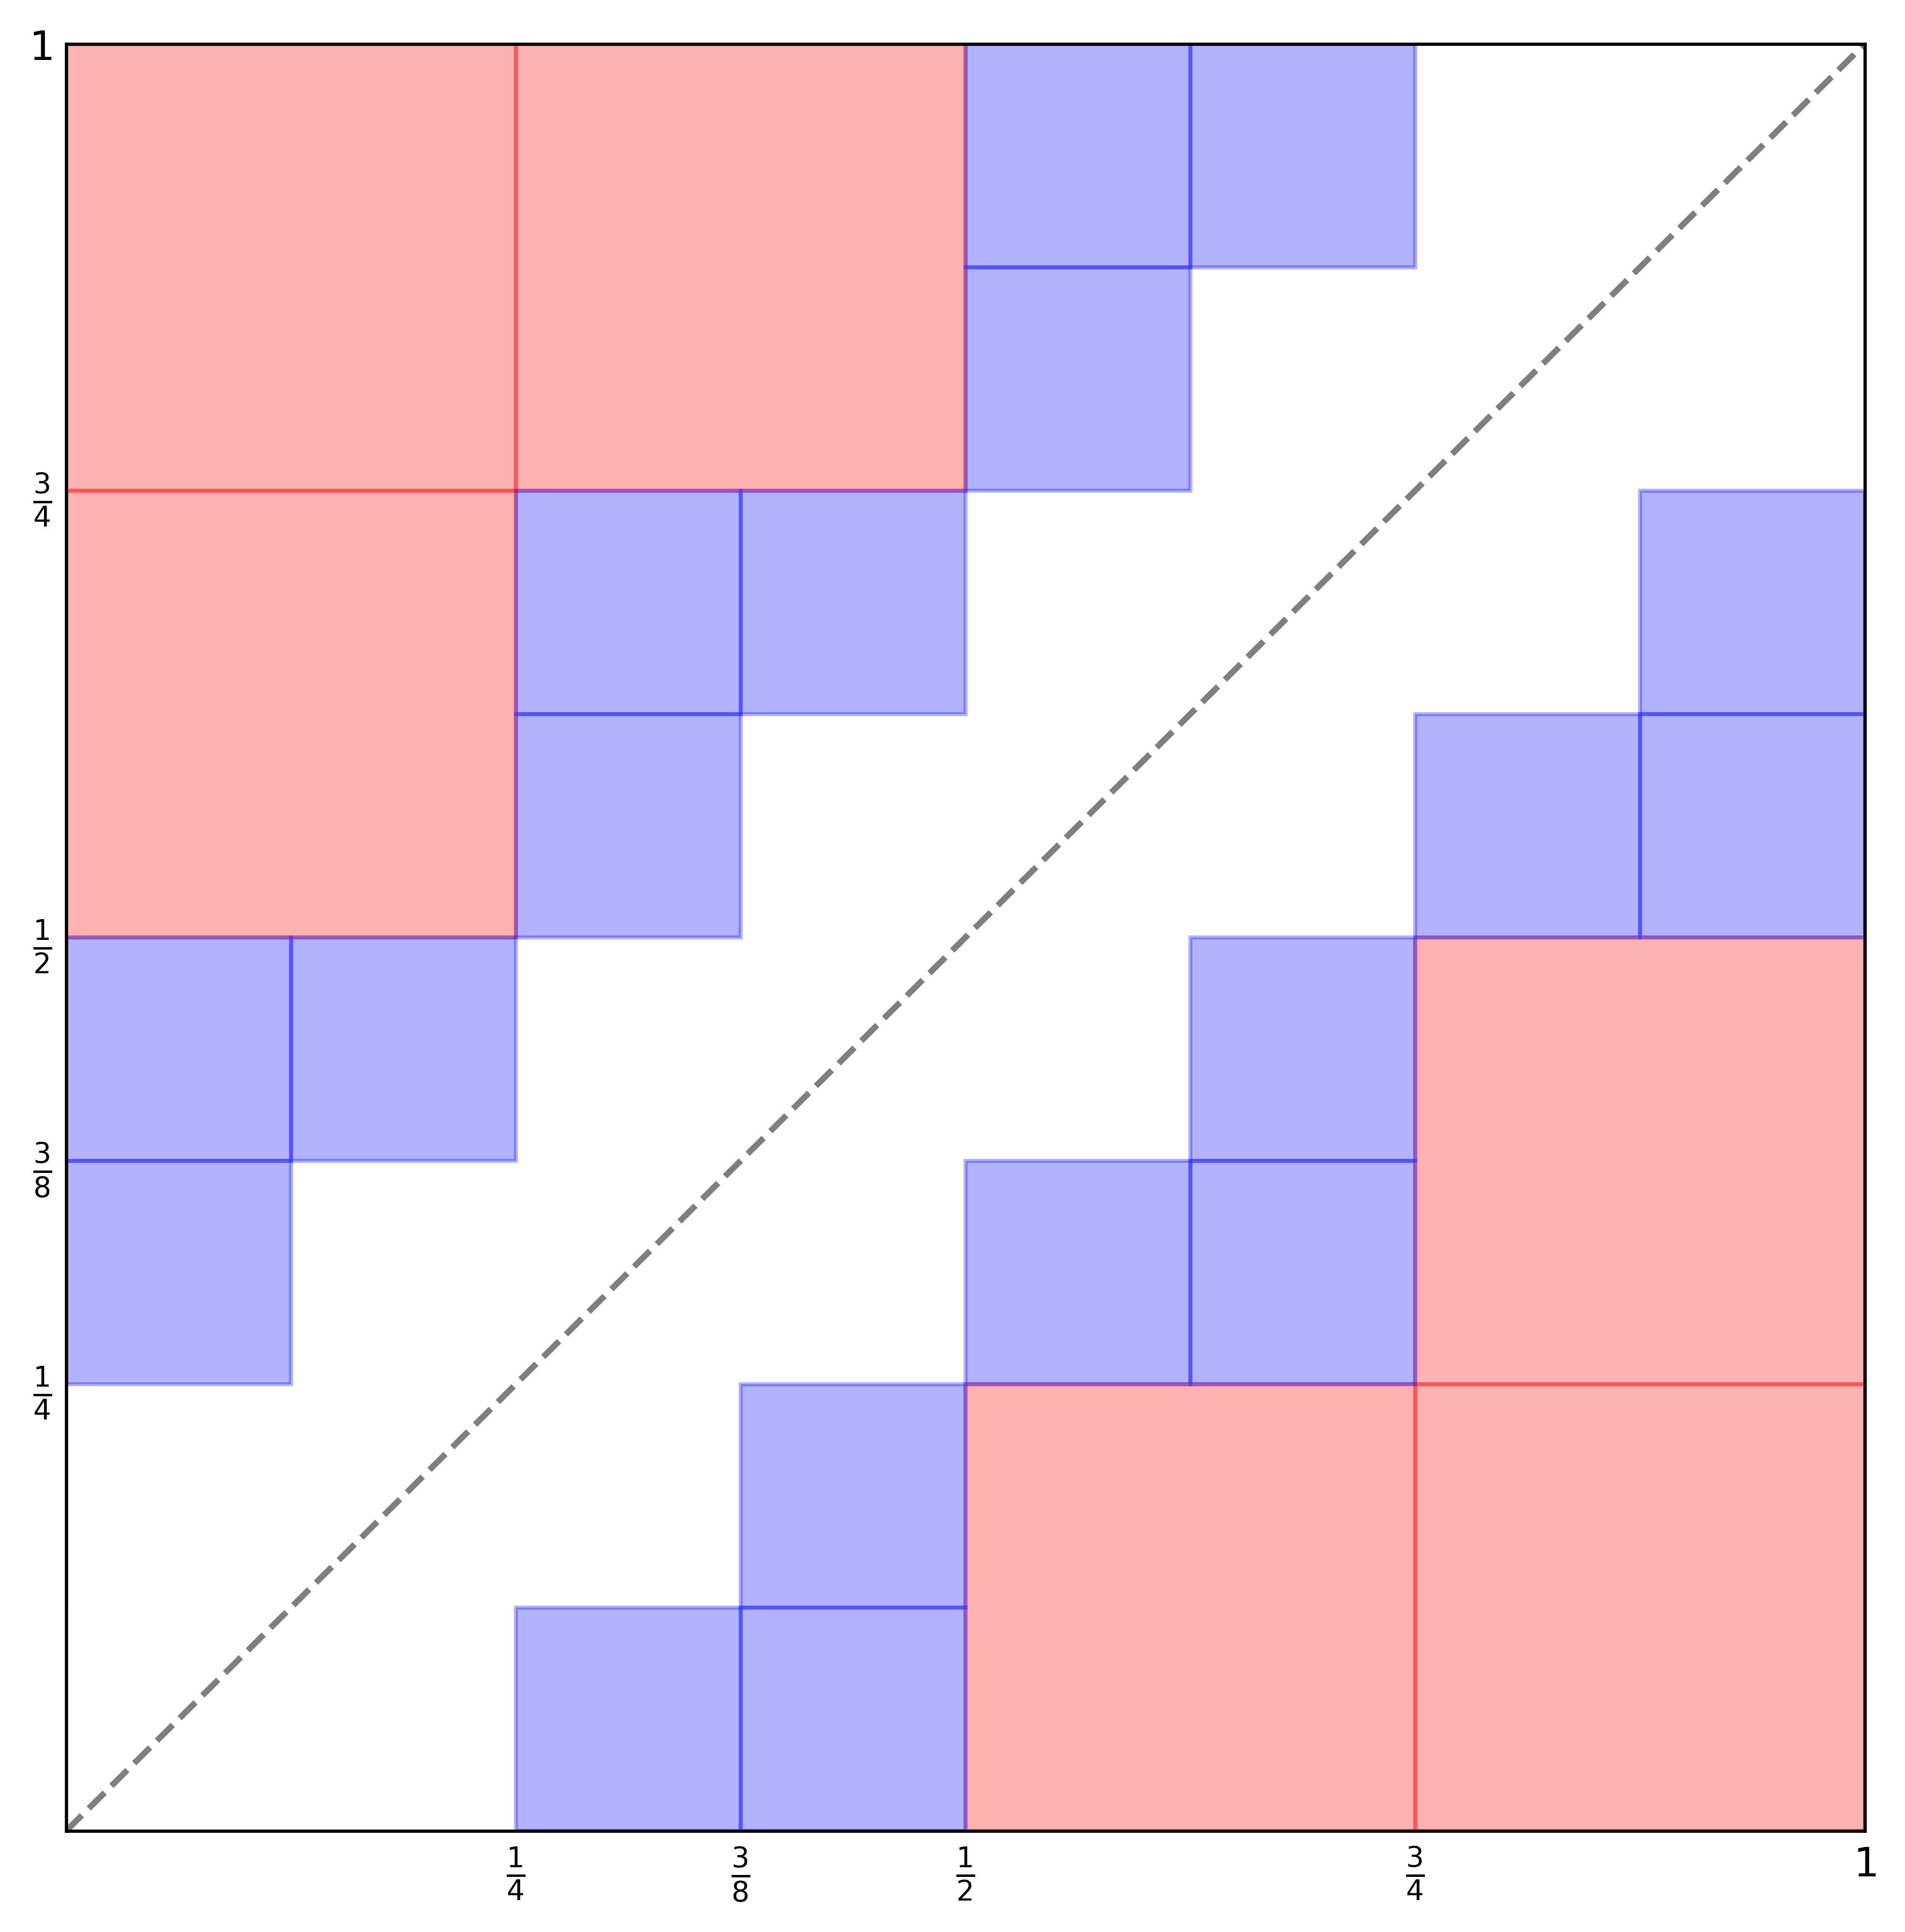
\includegraphics[scale=0.5]{/home/dnf/Downloads/Thesis/Chapters/General curve/whitney_decomp.png}
    \caption{Whitney decompostion}
    \label{fig:whitney}
\end{figure}


\begin{lem}
 Let $I \in \mathcal{P}\left(2^{-n}\right)$ for some integer $n \geqslant 0$. For any $\delta \in\left(0,2^{-n}\right)$ and any tuple of functions $\left(f_{J}\right)_{J \in \mathcal{P}(I, \delta)}$ with $\operatorname{supp} \widehat{f_{J}} \subseteq \mathcal{U}_{J}$ for all $J$, the following inequality holds:


\begin{equation*}
\left\|f_{I}\right\|_{p_{k}} \leqslant \mathcal{D}_{k}\left(2^{n} \delta\right)\left(\sum_{J \in \mathcal{P}(I, \delta)}\left\|f_{J}\right\|_{p_{k}}^{2}\right)^{1 / 2} 
\end{equation*}

Let $I, I^{\prime} \in \mathcal{P}\left(2^{-n}\right)$ for some integer $n \geqslant 2$ with $2^{n} \operatorname{dist}\left(I, I^{\prime}\right) \in\{1,2\}$. For any $\delta \in\left(0,2^{-n}\right)$ and any tuple of functions $\left(f_{J}\right)_{J \in \mathcal{P}(I, \delta) \cup \mathcal{P}\left(I^{\prime}, \delta\right)}$ with $\operatorname{supp} \widehat{f_{J}} \subseteq \mathcal{U}_{J}$ for all $J$, the following inequality holds:


\begin{equation*}
\int_{\mathbb{R}^{k}}\left|f_{I}\right|^{p_{k} / 2}\left|f_{I^{\prime}}\right|^{p_{k} / 2} \leqslant \mathcal{B}\left(2^{n-2} \delta\right)^{p_{k}}\left[\sum_{J \in \mathcal{P}(I, \delta)}\left\|f_{J}\right\|_{p_{k}}^{2}\right]^{p_{k} / 4}\left[\sum_{J^{\prime} \in \mathcal{P}\left(I^{\prime}, \delta\right)}\left\|f_{J^{\prime}}\right\|_{p_{k}}^{2}\right]^{p_{k} / 4} 
\end{equation*}
\end{lem}
\begin{proof}
    See where to prove this. Here or in chapter 2. (It's the same thing)
\end{proof}
\begin{proof}[Proof of Lemma \ref{lem:bil_redu}]
Suppose that $\delta=2^{-N}$. Set $\mathcal{W}_{1}:=\varnothing$. For integers $n \geqslant 2$, define iteratively

$$
\mathcal{W}_{n}:=\left\{\left(I_{1}, I_{2}\right) \in \mathcal{P}\left(2^{-n}\right) \mid 2^{n} \operatorname{dist}\left(I_{1}, I_{2}\right) \in\{1,2\} \text { and } I_{1} \times I_{2} \notin \bigcup_{\left(I_{1}^{\prime}, I_{2}^{\prime}\right) \in \mathcal{W}_{n-1}} I_{1}^{\prime} \times I_{2}^{\prime}\right\}
$$

For each $n\geq2$, $\mathcal{W}_n$ contains the squared of side length $2^{-n}$ present in the decomposition. Since we are only interested in information about the norms up to scale $2^{-N}$ we need to stop the decomposition at this stage. To turn this into partition of $[0,1]^2$ had the diagonal pieces at scale $2^{-N}$,


$$
\widetilde{\mathcal{W}}_{N}:=\left\{\left(I_{1}, I_{2}\right) \in \mathcal{P}\left(2^{-N}\right) \mid \operatorname{dist}\left(I_{1}, I_{2}\right)=0\right\}.
$$

Then, 

$$
\mathcal{W}^{N}:=\bigcup_{n=2}^{N} \mathcal{W}_{n} \cup \widetilde{\mathcal{W}}_{N}
$$

form an essentially disjoint (up to boundaries) covering of $[0,1]^{2}$. Let $\left(f_{J}\right)_{J \in \mathcal{P}(\delta)}$ be as in Definition \ref{defn:gen_moment} for $\mathcal{D}_{k}(\delta)$. Then


\begin{align*}
\left\|\sum_{J \in \mathcal{P}(\delta)} f_{J}\right\|_{p_{k}} & =\left\|\sum_{\left(I, I^{\prime}\right) \in \mathcal{W}^{N}} f_{I} \overline{f_{I^{\prime}}}\right\|_{p_{k} / 2}^{1 / 2} \leqslant\left(\sum_{\left(I, I^{\prime}\right) \in \mathcal{W}^{N}}\left\|f_{I} \overline{f_{I^{\prime}}}\right\|_{p_{k} / 2}\right)^{1 / 2} \\
& \leqslant\left(\sum_{\left(I, I^{\prime}\right) \in \widetilde{\mathcal{W}}_{N}}\left\|f_{I}\right\|_{p_{k}}\left\|f_{I^{\prime}}\right\|_{p_{k}}+\sum_{n=2}^{N} \sum_{\left(I, I^{\prime}\right) \in \mathcal{W}_{n}}\left\|f_{I} \overline{f_{I^{\prime}}}\right\|_{p_{k} / 2}\right)^{1 / 2}
\end{align*}

We estimate the first term by

$$
\sum_{I, I^{\prime} \in  \widetilde{\mathcal{W}}_{N}}\left(\left\|f_{I}\right\|_{p_{k}}^{2}+\left\|f_{I^{\prime}}\right\|_{p_{k}}^{2}\right) \leqslant 6 \sum_{I \in \mathcal{P}\left(2^{-N}\right)}\left\|f_{I}\right\|_{p_{k}}^{2}
$$

since each $I$ appears at most 6 times in the pairs $\widetilde{\mathcal{W}}_{N}$. In the second term, by affine rescaling (), for every $\left(I, I^{\prime}\right) \in \mathcal{W}_{n}$, we have

\[
\begin{aligned}
\left\|f_{I} \overline{f_{I^{\prime}}}\right\|_{p_{k} / 2} & \lesssim \mathcal{B}\left(2^{-N+n-2}\right)^{2} \left( \ell_{J \in \mathcal{P}(I, 2^{-N})}^{2} \left\|f_{J}\right\|_{p_{k}} \right) \left( \ell_{J^{\prime} \in \mathcal{P}(I^{\prime}, 2^{-N})}^{2} \left\|f_{J^{\prime}}\right\|_{p_{k}} \right) \\
& \lesssim \mathcal{B}\left(2^{-N+n-2}\right)^{2} \left(\left( \ell_{J \in \mathcal{P}(I, 2^{-N})}^{2} \left\|f_{J}\right\|_{p_{k}} \right)^{2} + \left( \ell_{J^{\prime} \in \mathcal{P}(I^{\prime}, 2^{-N})}^{2} \left\|f_{J^{\prime}}\right\|_{p_{k}} \right)^{2} \right)
\end{aligned}
\]


Since each $I \in \mathcal{P}\left(2^{-n}\right)$ appears at most 8 times in $\mathcal{W}_{n}$, it follows that

$$
\sum_{\left(I, I^{\prime}\right) \in \mathcal{W}_{n}}\left\|f_{I} \overline{f_{I^{\prime}}}\right\|_{p_{k} / 2} \lesssim \mathcal{B}\left(2^{-N+n-2}\right)^{2}\left( \ell_{J \in \mathcal{P}(2^{-N})}^{2} \left\|f_{J}\right\|_{p_{k}} \right)
$$

Inserting these bounds in (2.5), we obtain the desired estimate.
\end{proof}

\subsection{Main object}
In this subsection we develop the essential ingredients for the main object of study. We start by introducing some standard... 

Introduce the $k$ bilinear objects and essencially reproduce the averaging argument done in (chapter 2). That approach heavly relies of the uncertaintly principle, so we need to formalize it in the context of this problem.
For a dyadic interval $I$, let $\freqU_{I}$ denote the parallelepiped centered at the origin dual to $\calU_{I}$, that is,

$$
\freqU_{I}:=\left\{\left.x \in \mathbb{R}^{k}:|\left\langle x, \partial^{i} \Gamma\left(c_{I}\right)\right\rangle|\leqslant| I\right|^{i}, 1 \leqslant i \leqslant k\right\}.
$$



Here, \( A \) represents a dimensional constant with specific requirements: \( A > k \) and \( A \geqslant \frac{k(k+1)}{2} \). One can interpret \( \phi_{I} \) as a smoother version of the indicator function \( |\freqU_{I}|^{-1}\mathrm{1}_{\freqU_{I}} \), remaining constant inside \( \freqU_{I} \) and decaying rapidly outside. Lemmas A.1 and A.2 provide further insights into why these conditions are necessary for the decay behavior of \( \phi_{I} \). Furthermore, one can see that the $L^1$ norm is independent of the chosen interval.\\

Let \( M_{I} \) and \( \phi \) be defined in the following way:

\begin{equation}\label{eq:change_box}
M_{I} = \left[ \begin{array}{c|c|c|c}
\partial^1 \Gamma(c_{I}) & \partial^2 \Gamma(c_{I}) & \cdots & \partial^k \Gamma(c_{I})
\end{array} \right]
\end{equation}

and 

\begin{equation}\label{eq:function_change_box}
\phi_{\delta}(x)= \delta^{k(k+1)/2} \max \{1, \delta |x_1|, \cdots, \delta^{k} |x_k|\}^{-A}.
\end{equation}

Observing that \(\langle (M_{I}^{-1})^{\top} x, \partial^i \Gamma \rangle = \langle x, M_{I}^{-1} \partial^i \Gamma \rangle = \langle x, e_i \rangle\), the following can be seen as an expression invariant under the choice of interval after an elementary change of variables:

\[
\int_{\R^k} \phi_{I}(x)\, dx = \int_{\R^k} \phi_{I}((M^{-1})^{\top} x)\, dx = \int_{\R^k} \phi_{\delta}(x)\, dx.
\]

\begin{lem}[Uncertaintly principle]\label{lem:uncer.prin.}
    For $p \in[1, \infty)$ and $J \subset[0,1]$, we have

$$
\left|g_{J}\right|^{p} \lesssim_{p}\left|g_{J}\right|^{p} * \phi_{J}
$$

for every $g_{J}$ with $\operatorname{supp} \widehat{g_{J}} \subseteq C \mathcal{U}_{J}$.

\end{lem}
\begin{proof}
Let $\psi$ be a Schwartz function adapted to $\mathcal{U}_{J}^{\circ}$ such that $\hat{\psi} \equiv 1$ on $C \mathcal{U}_{J}$ and $\int|\psi| \approx 1$. Then $g_{J}=g_{J} * \psi$, so


\begin{align*}
\left|g_{J}\right|^{p}(x) & \leqslant\left(\int\left|g_{J}(x-z)\right|^{p}|\psi(z)| \mathrm{d} z\right)\left(\int|\psi(z)| \mathrm{d} z\right)^{p / p^{\prime}}\\
& \lesssim\left(\left|g_{J}\right|^{p} *|\psi|\right)(x) \lesssim\left(\left|g_{J}\right|^{p} * \phi_{J}\right)(x)
\end{align*}

\end{proof}
As a mater of fact, under the support hypothesis of (\ref{lem:uncer.prin.}) the function $\left|g_{J}\right|^{p} * \phi_{J}$ rigorously satisfies the heuristic of being essentially constant on translates of the dual box. Define
$$\mathcal{U}_{\delta} =\{x\in \R^k\text{: } \forall i\text{, } |x_i|\leq \delta^{i} \}, $$ then $x\in \mathcal{U}_{\delta}$ if and only if $(M_{J})^{\top}x \in \freqU_{J}$.
Take $x \in \mathcal{U}_{\delta}$ and proceed as above to obtain 
$$\left|g_{J}\right|^{p} * \phi_{J}((M_{J}^{-1})^{\top}x_{1}) = \int_{\R^k} |g_{J}|^{p}(y)\phi_{J}((M_{J}^{-1})^{\top}x_{1}-y)dy \sim 
\int_{\R^k} |g_{J}|^{p}((M_{J}^{-1})^{\top}y)\phi_{J}((M_{J}^{-1})^{\top}(x_{1}-y))dy. 
$$
By using an analogous formula to \ref{eq:function_change_box}, one can see that for $x_1$ $x_2$ $\in \mathcal{U}_\delta$, $$\left|g_{J}\right|^{p} * \phi_{J}((M_{J}^{-1})^{\top}x_{1}) \sim \left|g_{J}\right|^{p} * \phi_{J}((M_{J}^{-1})^{\top}x_{2}),$$ with absolute constant independent of the size of $J$.

Motivated by this formulation of the uncertainly principle we now define the main objects of study in the following way:

\begin{defn}\label{def:assymetric}
     For $l \in\{0, \ldots, k-1\}, a, b \in[0,1]$ and $\delta \in(0,1)$, 
     the (asymmetric) bilinear decoupling constant $\mathcal{B}_{l, a, b}(\delta)$ for the moment curve 
     $\Gamma$ in $\hat{\mathbb{R}}^{k}$ is the smallest constant such that, 
     for all pairs of intervals $I \in \mathcal{P}\left(\delta^{a}\right), I^{\prime} \in \mathcal{P}\left(\delta^{b}\right)$
      with $\operatorname{dist}\left(I, I^{\prime}\right) \geqslant 1 / 4$ and all tuples of functions 
      $\left(f_{J}\right)_{J \in \mathcal{P}(I, \delta) \cup \mathcal{P}\left(I^{\prime}, \delta\right)}$
       with supp $\widehat{f_{J}} \subseteq \mathcal{U}_{J}$ for all $J$, the following inequality holds:


\begin{align*}
& \int_{\mathbb{R}^{k}}\left(\left|f_{I}\right|^{p_{l}} * \phi_{I}\right)\left(\left|f_{I^{\prime}}\right|^{p_{k}-p_{l}} * \phi_{I^{\prime}}\right) \\
& \leqslant \mathcal{B}_{l, a, b}(\delta)^{p_{k}}\left[\sum_{J \in \mathcal{P}(I, \delta)}\left\|f_{J}\right\|_{p_{k}}^{2}\right]^{p_{l} / 2}\left[\sum_{J^{\prime} \in \mathcal{P}\left(I^{\prime}, \delta\right)}\left\|f_{J^{\prime}}\right\|_{p_{k}}^{2}\right]^{\left(p_{k}-p_{l}\right) / 2} 
\end{align*}

\end{defn}

\begin{rmk}
     In the case $l=0$, the bilinear decoupling constant $\mathcal{B}_{0, a, b}(\delta)$  does not depend on $a$, by using affine rescaling (citar affine rescaling), we have


\begin{equation*}
\mathcal{B}_{0, a, b}(\delta) \sim \mathcal{D}_{k}\left(\delta^{1-b}\right).
\end{equation*}

\end{rmk}

\begin{lem}\label{lem:sym.to.asym.}
For every $l \in\{0, \ldots, k-1\}, a, b \in[0,1]$ and $\delta \in(0,1 / 4)$, we have

\begin{equation*}
\mathcal{B}(\delta) \lesssim \delta^{-a p_{l} / p_{k}} \delta^{-b\left(p_{k}-p_{l}\right) / p_{k}} \mathcal{B}_{l, a, b}(\delta) \tag{3.4}
\end{equation*}

\end{lem}

\begin{proof}
    Let $I, I^{\prime} \in \mathcal{P}(1 / 4)$ with $\operatorname{dist}\left(I, I^{\prime}\right) \geqslant 1 / 4$. Let $\left(f_{K}\right)_{K \in \mathcal{P}(I, \delta) \cup \mathcal{P}\left(I^{\prime}, \delta\right)}$ be a tuple of functions with supp $\widehat{f_{K}} \subseteq \mathcal{U}_{K}$ for all $K$. By Hölder's inequality, we have


\begin{equation*}
\int_{\mathbb{R}^{k}}\left|f_{I}\right|^{p_{k} / 2}\left|f_{I^{\prime}}\right|^{p_{k} / 2} \leqslant\left(\int_{\mathbb{R}^{k}}\left|f_{I}\right|^{p_{l}}\left|f_{I^{\prime}}\right|^{p_{k}-p_{l}}\right)^{1 / 2}\left(\int_{\mathbb{R}^{k}}\left|f_{I}\right|^{p_{k}-p_{l}}\left|f_{I^{\prime}}\right|^{p_{l}}\right)^{1 / 2} \tag{3.5}
\end{equation*}


By symmetry, it suffices to estimate the first bracket. Assume that $l \neq 0$; the case $l-0$ is similar, but easier, since the term with power $p_{l}$ disappears. We have

$$
\begin{aligned}
\int_{\mathbb{R}^{k}}\left|f_{I}\right|^{p_{l}}\left|f_{I^{\prime}}\right|^{p_{k}-p_{l}} & \leqslant \int_{\mathbb{R}^{k}}\left(\sum_{J \in \mathcal{P}\left(I, \delta^{a}\right)}\left|f_{J}\right|\right)^{p_{l}}\left(\sum_{J^{\prime} \in \mathcal{P}\left(I^{\prime}, \delta^{b}\right)}\left|f_{J^{\prime}}\right|\right)^{p_{k}-p_{l}} \\
& \leqslant\left|\mathcal{P}\left(I, \delta^{a}\right)\right|^{p_{l}-1}\left|\mathcal{P}\left(I^{\prime}, \delta^{b}\right)\right|^{p_{k}-p_{l}-1} \sum_{J \in \mathcal{P}\left(I, \delta^{a}\right)} \sum_{J^{\prime} \in \mathcal{P}\left(I^{\prime}, \delta^{b}\right)} \int_{\mathbb{R}^{k}}\left|f_{J}\right|^{p_{l}}\left|f_{J^{\prime}}\right|^{p_{k}-p_{l}}
\end{aligned}
$$

By Lemma 3.3 and Definition 3.1, we have

$$
\begin{aligned}
\int_{\mathbb{R}^{k}}\left|f_{J}\right|^{p_{l}}\left|f_{J^{\prime}}\right|^{p_{k}-p_{l}} & \lesssim \int_{\mathbb{R}^{k}}\left(\left|f_{J}\right|^{p_{l}} * \phi_{J}\right)\left(\left|f_{J^{\prime}}\right|^{p_{k}-p_{l}} * \phi_{J^{\prime}}\right) \\
& \leqslant \mathcal{B}_{l, a, b}(\delta)^{p_{k}}\left[\ell_{K \in \mathcal{P}(J, \delta}^{2}\left\|f_{K}\right\|_{p_{k}}\right]^{p_{l}}\left[\ell_{K^{\prime} \in \mathcal{P}\left(J^{\prime}, \delta\right)}^{2}\left\|f_{K^{\prime}}\right\|_{p_{k}}\right]^{p_{k}-p_{l}}
\end{aligned}
$$

Inserting this into the previous display, and using $\ell^{2} \hookrightarrow \ell^{p_{l}}, \ell^{p_{k}-p_{l}}$, we obtain

$$
\begin{aligned}
\int_{\mathbb{R}^{k}}\left|f_{I}\right|^{p_{l}}\left|f_{I^{\prime}}\right|^{p_{k}-p_{l}} \lesssim \delta^{-a\left(p_{l}-1\right)} \delta^{-b\left(p_{k}-p_{l}-1\right)} \mathcal{B}_{l, a, b}(\delta)^{p_{k}} \\
\cdot\left[\ell_{K \in \mathcal{P}(I, \delta)}^{2}\left\|f_{K}\right\|_{p_{k}}\right]^{p_{l}}\left[\ell_{K^{\prime} \in \mathcal{P}\left(I^{\prime}, \delta\right)}^{2}\left\|f_{K^{\prime}}\right\|_{p_{k}}\right]^{p_{k}-p_{l}}
\end{aligned}
$$

Together with a similar estimate for the second factor in (3.5), we obtain the desired estimate.
\end{proof}


\subsection{Capturing the tranversality}
As discussed in the chapter on the (Parabola), we simplified the study of the decoupling constant to focus on a bilinear object.
In fact, the final iteration crucially relies on the key result Theorem (0.3.2), which enables the iteration process. 
Furthermore, the same picture as guide for this results can also serve as a blueprint for this higher-dimensional case.

In essence, we picked a particular one-dimensional linear subspace, projected the curve onto it, and observed that the resulting curve behaved
as a straight line. 
In this scenario, this can be interpreted as the 0-dimensional moment curve, where the decoupling results are straightforwardly Plancherel.
This same scenario repeats in higher dimensions. By picking the appropriate subspaces, we can see that the projections 
of the curve resemble lower-dimensional versions, making it possible to use lower-degree decoupling to obtain sharp estimates for 
the asymetric bilinear object.

By choosing to work with higher order tangent spaces and their orhtogonal complement the argument becames quite clean.
\begin{defn}
    Let $V^{(l)}(\xi)$ denote the $l$-th order tangent space to the moment curve $\Gamma$ at the point $\xi$, that is, 
    \begin{equation*}
        V^{(l)}(\xi):= Span\{ \partial^1 \Gamma(\xi),\cdots,\partial^l \Gamma(\xi)\}.
    \end{equation*}
\end{defn}
\begin{rmk}
    These same spaces are considered in the original Bourgain-Guth-Demeter proof but in the context of Kakeya-Brascamp-Lieb type inequalities, 
    a topic that wasn't explored. For more details, see [Pavel, Section 9]. 
\end{rmk}

The following auxiliary result quantifies the tranversality between distinct higher order tangent spaces. The proof relies on the generalized Vandermonde
determinant formula in [Kat84, Equation (14)], and can be see in [Short proof].

\begin{lem}
For any integers $0 \leqslant l \leqslant k$ and any $\xi_{1}, \xi_{2} \in \mathbb{R}$, we have
    \begin{equation*}
    \left|\partial^{1} \Gamma\left(\xi_{1}\right) \wedge \cdots \wedge \partial^{l} \Gamma\left(\xi_{1}\right) \wedge \partial^{1} \Gamma\left(\xi_{2}\right) \wedge \cdots \wedge \partial^{k-l} \Gamma\left(\xi_{2}\right)\right| \gtrsim_{k, l}\left|\xi_{1}-\xi_{2}\right|^{l(k-l)} \tag{3.6}
    \end{equation*}
\end{lem}

As an auxiliary result, we need a result about decoupling for a more general class of curves.
 This can be seen as a prototypical situation where inequalities are proved for model manifolds and then extended to similarly 
 curved manifolds (see [Dem]). The argument presented here is based on the one given in [BD15, Section 7], 
 with extra steps due to the differences in the neighborhoods considered.

 Suppose $l \in \mathbb{N}$ and $\gamma:[0,1] \rightarrow \hat{\mathbb{R}}^{l}$ is a curve such that


 \begin{equation*}
 \|\gamma\|_{C^{l+1}} \lesssim 1 \quad \text { and } \quad\left|\partial^{1} \gamma(\xi) \wedge \cdots \wedge \partial^{l} \gamma(\xi)\right| \gtrsim 1 \tag{3.7}
 \end{equation*}
 
 For dyadic intervals $J$, let $\mathcal{U}_{J, \gamma}$ be the parallelepiped of dimensions $|J|^{1} \times \cdots \times|J|^{l}$
  whose center is $\gamma\left(c_{J}\right)$ and sides are parallel to
   $\partial^{1} \gamma\left(c_{J}\right), \ldots, \partial^{l} \gamma\left(c_{J}\right)$, 
   and let $\mathcal{U}_{J, \gamma}^{\circ}$ be polar to $\mathcal{U}_{J, \gamma}$.


   
\begin{lem}\label{lem:lower_degree_decoupling}
 Suppose that Theorem 1.2 is known with $k$ replaced by $l$. Let $\gamma:[0,1] \rightarrow \mathbb{R}^{l}$ be a curve satisfying
  (condicoes para curva gamma). Then for any $\epsilon, C>0$,
   any $\delta \in(0,1)$, and any tuple of functions 
   $\left(f_{J}\right)_{J \in \mathcal{P}(\delta)}$ with $\operatorname{supp} \widehat{f_{J}} \subseteq C \mathcal{U}_{J, \gamma}$ for all $J$, 
   the following inequality holds:

\begin{equation}
    \norm{ \sum_{J \in \Part(\delta)} f_{J} }_{\lpl}
    \lesssim_{\varepsilon, C}\delta^{-\varepsilon}
    \Bigl( \sum_{J \in \Part(\delta)} \norm{ f_{J} }_{\lpl}^{2} \Bigr)^{1/2}.
\end{equation}
\end{lem}
\begin{proof}
    Let $\left(f_{J}\right)_{J \in \mathcal{P}(\delta)}$ be a tuple of functions with supp
     $\widehat{f_{J}} \subseteq C \mathcal{U}_{J, \gamma}$ for all $J$. The proof exploits the iterative nature of 
     decoupling inequalities. Assume that for every $\kappa>\delta^{l /(l+1)}$ and $I \in \mathcal{P}(\kappa)$,
    we have
    \begin{equation}\label{eq:iter_eq}
        \norm{f_I}_{\lpl} \lesssim_{\varepsilon} \ell^{2}_{I^{\prime}\in \Part(I,\kappa^{(l+1)/l})}
        \norm{f_{I^{\prime}}}_{\lpl}.
    \end{equation}
    Let $M$ be large interger to be choosen later, then by Cauchy-Schwartz,
    \begin{equation}
    \norm{f}_{\lpl}\lesssim \Dec(\scale{M}) \Bigl( \sum_{I \in \Part(\delta)} \norm{ f_{I} }_{\lpl}^{2} \Bigr)^{1/2}
    \lesssim \delta^{-\frac{1}{2}\left(\frac{l}{l+1}\right)^{M}} \Bigl( \sum_{I \in \Part(\delta)} \norm{ f_{I} }_{\lpl}^{2} \Bigr)^{1/2}
    \end{equation}
     by applying (\ref{eq:iter_eq}) yields:

     \begin{equation}
        \lesssim \delta^{-\frac{1}{2}\left(\frac{l}{l+1}\right)^{M}} \Bigl( \sum_{I \in \Part(\delta)} \sum_{I^{\prime} \in \Part(\delta)} 
        \delta^{-\frac{1}{2}\left(\frac{l}{l+1}\right)^{M}\varepsilon}\;\norm{ f_{I^{\prime}} }_{\lpl}^{2} \Bigr)^{1/2}
     \end{equation}
     \begin{equation}
        = \delta^{-\frac{1}{2}\left(\frac{l}{l+1}\right)^{M}} \delta^{-\frac{1}{2}\left(\frac{l}{l+1}\right)^{M}\varepsilon}
        \Bigl( \sum_{I \in \Part\left(\delta^{\left(\frac{l}{l+1}\right)^{M}}\right)} \norm{ f_{I} }_{\lpl}^{2} \Bigr)^{1/2}.
     \end{equation}
     By iteraring $M$ times,
     \begin{equation}
        \norm{f}_{\lpl} \lesssim_{\varepsilon} \delta^{-\frac{1}{2}\alpha(l,M,\varepsilon)} \Bigl( \sum_{J \in \Part(\delta)} \norm{ f_{J} }_{\lpl}^{2} \Bigr)^{1/2}
     \end{equation}
     where 
     $$\alpha(l,M,\varepsilon)= \left(\frac{l}{l+1}\right)^{M}+ \left[ 1 - \left(\frac{l}{l+1}\right)^{M} \right](l+1)\varepsilon$$
     since $M$ is arbitrary this concludes the proof.

     To see why (\ref{eq:iter_eq}) is true consider that on $I\in \Part(\kappa)$ we have
     \begin{equation}
        \gamma(\xi) = \underbrace{\gamma\left(c_{I}\right) + \partial^{1} \gamma\left(c_{I}\right) \cdot (\xi - c_{I}) + \cdots + \frac{\partial^{l} \gamma\left(c_{I}\right)}{l!} \cdot (\xi - c_{I})^{l}}_{\substack{P_{I,l}(\xi)}} + O\left(\kappa^{l+1}\right).     
    \end{equation}
    By (cond gamma) $P_{I,l}$ is up to uniforme non-singular affine transformation a moment curve of degree $l$.
    Since the decoupling constant is invariant under this type of transformations, assuming the validity of Theorem () with $l$ instead of $k$, 
      Lemma \ref{lem:lower_degree_decoupling} is true for $\gamma = P_{I,l}$. Moreover, one can get the analogous of (\ref{eq:iter_eq})
     for free since it's merely a rescaled version. 
     
    So, if one can show that for $I^{\prime}\in \Part(\kappa^{\frac{l+1}{l}})$ 
    there exists a absolute constant $C'>0$ such that $\calU_{I^{\prime},\gamma}\subseteq C^{'}\calU_{I^{\prime}, P_{I,l}}$, then (\ref{eq:iter_eq})
     is true. For that calculation see appendix (). 
\end{proof}
\begin{cor}
 In the situation of Lemma 3.6, for any $A^{\prime}>0$ and for every ball $B \subset \mathbb{R}^{l}$ of radius $\delta^{-l}$, we have

$$
\fint_{B}\left|\sum_{J \in \mathcal{P}(\delta)} f_{J}\right|^{p_{l}} \lesssim_{\epsilon, C, A^{\prime}} \delta^{-\epsilon}\left(\ell_{J \in \mathcal{P}(\delta)}^{2}\left\|f_{J}\right\|_{L^{p_{l}\left(\Phi_{B}\right)}}\right)^{p_{l}}
$$

where $\fint_{B}:=|B|^{-1} \int_{B}$ denotes the average integral and

$$
\Phi_{B}(x):=|B|^{-1}\left(1+\delta^{l} \operatorname{dist}(x, B)\right)^{-A^{\prime}}
$$

is an $L^{1}$ normalized bump function adapted to $B$.
\end{cor}
\begin{proof}
 Apply Lemma 3.6 to functions $f_{J} \psi_{B}$, where $\psi_{B}$ is a Schwartz function such that $\left|\psi_{B}\right| \sim 1$ on $B$ and $\operatorname{supp} \widehat{\psi_{B}} \subseteq B\left(0, \delta^{l}\right)$.

We will use Corollary 3.7 with $A^{\prime}:=A+k-2$, where $A$ is the exponent occurring in the definition of $\phi_{I}$. The choice of the exponent $A^{\prime}$ ensures that Lemma A. 2 holds.
\end{proof}

We now reach the crucial step analogous to Theorem 0.3.2. 

\section{From Diophatine system to expoential sums}
One of the most famous problems in number theory is the one of Waring: for each $k \geq 2$, is there an $s=s(k)$ such that every positive integer $N$ may be expressed as
\begin{equation}
N=x_{1}^{k}+\cdots+x_{s}^{k} ?
\end{equation}
Let $g(k)$ be the least integer $s$ having the property that all natural numbers are the sum of at most $s$ positive integral $k$-th powers.

The first instance of this question goes back to Lagrange, who proved that every integer can be written as the sum of four squares of integers. This result is sharp, as evidenced by the fact that 2023 cannot be written as the sum of three or fewer squares. To see this, consider the equation $x_{1}^2 + x_{2}^2 + x_{3}^2 \equiv 2023 \pmod{8}$; an exhaustive argument yields the desired conclusion. In a 1909 paper, Hilbert demonstrated via polynomial identities that $g(k) < \infty$. However, this approach does not provide much quantitative insight.

To address that one can consider a slightly different question, namely the number of representations of $N$ as the sum of $s$ $k$-th powers, denoted by $r_{s,k}(N)$. The idea hinges on the use of generating functions. Consider the series

$$
g_{k}(z)=\sum_{m=1}^{\infty} z^{m^{k}}
$$
which is is absolutely convergent for $|z|<1$.\\
If one now considers the expression $g_{k}(z)^{s}$, then 

$$
\begin{aligned}
g_{k}(z)^{s} & =\left(\sum_{m_{1}=1}^{\infty} z^{m_{1}^{k}}\right)\left(\sum_{m_{2}=1}^{\infty} z^{m_{2}^{k}}\right) \cdots\left(\sum_{m_{s}=1}^{\infty} z^{m_{s}^{k}}\right) \\
& =\sum_{m_{1}=1}^{\infty} \ldots \sum_{m_{s}=1}^{\infty} z^{m_{1}^{k}+\ldots+m_{s}^{k}} \\
& =\sum_{n=1}^{\infty} r_{s, k}(n) z^{n}
\end{aligned}
$$

where we write

$$
r_{s, k}(n)=\operatorname{card}\left\{m_{1}, \ldots, m_{s} \in \mathbb{N}: m_{1}^{k}+\ldots+m_{s}^{k}=n\right\}.
$$

By resorting to Cauchy's integral formula we can recover $r_{s, k}(n)$:

$$
r_{s, k}(n)=\frac{1}{2 \pi i} \int_{\mathcal{C}} g_{k}(z)^{s} z^{-n-1} \mathrm{~d} z
$$

in which $\mathcal{C}$ denotes a circular contour, centred at 0, and with radius $r$ satisfying $0<r<1$. For $k=1$, the series can be explicitly computed as $g_{1}(z)=\frac{z}{1-z}$, and one can proceed with calculations to retrieve the coefficients. However, for $k>1$, this process isn't as straightforward.

Instead of working with this infinite series we can't in fact substitute it by a finite Fourier series.

Observe that, if $x_{1}^{k}+\ldots+x_{s}^{k}=N$, then $x_i \leq N^{1/k}$. Define $X=\floor{N^{1/k}}$ and
$$
f_{k}(\theta, X)=\sum_{1 \leqslant x \leqslant X} e\left(\theta x^{k}\right).
$$
We then have
$$
\begin{aligned}
f_{k}(\theta, X)^{s} & =\left(\sum_{1 \leqslant x_{1} \leqslant X} e\left(\theta x_{1}^{k}\right)\right) \ldots\left(\sum_{1 \leqslant x_{s} \leqslant X} e\left(\theta x_{s}^{k}\right)\right) \\
& =\sum_{1 \leqslant x_{1} \leqslant X} \cdots \sum_{1 \leqslant x_{s} \leqslant X} e\left(\theta\left(x_{1}^{k}+\ldots+x_{s}^{k}\right)\right) \\
& =\sum_{1 \leqslant m \leqslant s X^{k}} r_{s, k}^{*}(m) e(\theta m)
\end{aligned}
$$
where
$$
r_{s, k}^{*}(m)=\operatorname{card}\left\{m_{1}, \ldots, m_{s} \in \mathbb{N} \cap[1, X]: m_{1}^{k}+\ldots+m_{s}^{k}=m\right\}
$$
Thus, by applying the orthogonality relation
$$
\int_{0}^{1} e(\theta h) \mathrm{d} \theta= \begin{cases}0, & \text { when } h \in \mathbb{Z} \backslash\{0\} \\ 1, & \text { when } h=0\end{cases}
$$
we deduce that 
$$
\int_{0}^{1} f_{k}(\theta, X)^{s} e(-\theta N) d \theta=\sum_{1 \leqslant m \leqslant s X^{k}} r_{s, k}^{*}(m) \int_{0}^{1} e(\theta(m-N)) d \theta=r_{s, k}(N).
$$
So, to understand \( r_{s, k} \), we need to better understand \( f_k \). Furthermore, the even powers of \( f_k \) also encode number theoretical information about the Waring problem. Namely,
$$
\int_{0}^{1}\left|f_{k}(\theta, X)\right|^{2s} d \theta
$$
counts the number of solutions of the equation
\begin{equation}\label{Waring system}
x_{1}^{k}+\ldots+x_{s}^{k}=x_{s+1}^{k}+\ldots+x_{2s}^{k}
\end{equation}
for \(1 \leq x_{i} \leq X\). To see this, write \(\left|f_{k}(\theta, X)\right|^{2s} = f_{k}(\theta, X)^{s} \cdot \overline{f_{k}(\theta, X)}^{s}\) and explicitly compute the product. By using the orthogonality relation, the only exponentials that make a contribution are the ones where the exponent satisfies the condition \(x_{1}^{k} + \ldots + x_{s}^{k} - x_{s+1}^{k} - \ldots - x_{2s}^{k} = 0\). To further understand $f_k$ is the story of the circle method, which, for instance, allow to obtain an assymptic expansiton. In this section we don't stop to examine this function $f_{k}$, but instead define one more auxiliary function $J_{s, k}(X)$ which asymptotics we will study, for more details one the first approach see [Wooley, Circle].


For each integers $s \geq 1$ and $k, N \geq 2$ denote by $J_{s, k}(N)$ the number of integral solutions for the following system (called Vinogradov system)
\begin{equation}\label{Vinagradov system}
x_{1}^{\ell}+\ldots+x_{s}^{\ell}=x_{s+1}^{\ell}+\ldots+x_{2 s}^{\ell}, \quad(1 \leq \ell \leq k)
\end{equation}
with $1 \leq x_{i} \leq X$. Note first that for $J_{k, s}$ we have the identity
\begin{equation}\label{eq:J quatity solutions}
\int_{(0,1]^{k}}\left|F_{k}(\boldsymbol{\theta}, X)\right|^{2 s} d\boldsymbol{\theta}=J_{s, k}(X)
\end{equation}


where

$$
F_{k}(\boldsymbol{\alpha}, X)=\sum_{1 \leq x \leq X} e\left(\alpha_{1} x+\alpha_{2} x^{2}+\ldots+\alpha_{k} x^{k}\right)
$$

Identity (\ref{eq:J quatity solutions}) then follows in an identical fashion as when talking about $f_{k}$. Note then that we also have

$$
\int_{0}^{1}\left|f_{k}(\alpha, X)\right|^{2 s} \mathrm{~d} \alpha=\sum_{\left|h_{1}\right| \leq s X} \cdots \sum_{\left|h_{k}\right| \leq s X^{k-1}} \int_{(0,1]^{k}}\left|F_{k}(\boldsymbol{\alpha}, X)\right|^{2 s} e\left(-h_{1} \alpha_{1}-h_{2} \alpha_{2}-\ldots-h_{k-1} \alpha_{k-1}\right) \mathrm{d} \boldsymbol{\alpha}
$$

by a similar counting argument. By uniformly bounding the integral by $J_{k, s}$ and counting the number of terms in the above $(k-1)$-fold sum we see that

$$
\int_{0}^{1}\left|f_{k}(\alpha, X)\right|^{2 s} \mathrm{~d} \alpha \ll_{k, s} X^{\frac{k(k-1)}{2}} J_{s, k}(X).
$$

Relative to the Waring system, (\ref{Waring system}), the Vinogradov system (\ref{Vinagradov system}) displays more symmetries, namely translation-dilation invariance of solutions.
 Given real numbers \(\lambda\) and \(\xi\) with \(\lambda \neq 0\), the values \(x_{1}, \ldots, x_{2s}\) are solutions to the system

\begin{equation}\label{eq:Vinogradov 2}
\sum_{i=1}^{s} x_{i}^{j} = \sum_{i=1}^{s} x_{s+i}^{j} \quad 1 \leq j \leq k
\end{equation}

if and only if they are solutions to the system

$$
\sum_{i=1}^{s}\left(\lambda x_{i} + \xi\right)^{j} = \sum_{i=1}^{s}\left(\lambda x_{s+i} + \xi\right)^{j} \quad 1 \leq j \leq k.
$$

The invariance under \(\lambda\) can be seen as each equation is homogeneous of degree \(j\). Now, with \(\lambda = 1\), to understand the invariance under \(\xi \neq 0\), a computation gives

\begin{equation}\label{eq:vinogradov binomial}
\sum_{i=1}^{s}\left(\left(x_{i} + \xi\right)^{j} - \left(x_{s+i} + \xi\right)^{j}\right) = \sum_{\ell=1}^{j} \binom{j}{\ell} \xi^{j-\ell} \sum_{i=1}^{s} \left(x_{i}^{\ell} - x_{s+i}^{\ell}\right).
\end{equation}

If \(x_{1}, \ldots, x_{2s}\) are solutions to the system (\ref{eq:Vinogradov 2}), then each term in the inner sum on the right-hand side of (\ref{eq:vinogradov binomial}) vanishes, giving the desired conclusion.

The consequences of this are twofold. There are some implications in number theory, which can be seen in [LillianPierce] and from the point of view of decoupling for the moment curve, this can be seen as an important manifestation of the affine-rescaling property.
\subsection{Critical exponent}
When discussing Vinogradov's mean value theorem, it is often referred to as the main conjecture in this context. In this section, we will explore the reasons behind this designation.

To begin, we provide some bounds on \(J_{s, k}(N)\) from the perspective of solving the Vinogradov system. Notably, the diagonal solutions \(X_{j} = X_{s+j} \ (1 \leq j \leq s)\) are trivial solutions to the system. This observation gives us a straightforward lower bound: \(J_{s, k}(N) \geq N^{s}\). 

By considering the case where the sets \(\{X_{1}, \cdots, X_{s}\}\) and \(\{X_{s+1}, \cdots, X_{2s}\}\) are identical as multi-sets, we can slightly improve this lower bound to \(s!N^{s} + O(N^{s-1})\), [Wooley, ICM]. Furthermore, we establish the following upper bound:
\begin{lem}\label{lem:1st non trivial case}
     $J_{s, k}(N) \leq n!N^{2 s-n}$ when $s \geq n$.
\end{lem}
\begin{proof}
     The case $s \geq n$. Let $X_{n+1}, \cdots, X_{2 s}$ be chosen arbitrarily from $[N]$, then the value of $\sum_{j=1}^{n} X_{j}^{i}$ is fixed for each $1 \leq i \leq n$. So by Newton-Girard identities, all elementary symmetric functions of the $X_{1}, \cdots, X_{n}$ are determined and therefore $X_{j}$'s are determined up to their order. There are at most $n$ ! different permutations of $\left(X_{1}, \cdots, X_{n}\right)$, so $J_{s, k}(N) \leq n!N^{2 s-n}$.
\end{proof}

On the other hand, if we consider the analytic representation of $J_{s, k}(N)$, we get the trivial upper bound $N^{2 s}$. However, we can further improve this:

\begin{thm}
    $J_{s, k}(N) \gg N^{2 s-\frac{k(k+1)}{2}}$.
\end{thm}
\begin{proof}
 If $\left|\alpha_{j}\right| \leq \frac{1}{6 j N^{k}}$ for each $1 \leq j \leq k$, then we have

$$
\begin{gathered}
\left|\sum_{j=1}^{k} \alpha_{j} x^{j}\right| \leq \sum_{j=1}^{k}\left|\alpha_{j} x^{j}\right| \leq \sum_{j=1}^{k} \frac{1}{6 k}=\frac{1}{6} \\
\Re\left(e\left(\sum_{j=1}^{k} \alpha_{j} x^{j}\right)\right)=\cos \left(2 \pi\left(\sum_{j=1}^{k} \alpha_{j} x^{j}\right)\right) \geq \cos \left(\frac{\pi}{3}\right)=\frac{1}{2}
\end{gathered}
$$

Therefore,

$$
\left|F_{k}(\boldsymbol{\alpha}, N)\right|=\left|\sum_{1 \leqslant x \leqslant N}  e\left(\alpha_{1} x+\alpha_{2} x^{2}+\ldots+\alpha_{k} x^{k}\right)\right| \geq \sum_{1 \leqslant x \leqslant N}  \Re\left(e\left(\alpha_{1} x+\alpha_{2} x^{2}+\ldots+\alpha_{k} x^{k}\right)\right) \geq \frac{N}{2}
$$

So the analytic representation gives

$$
\begin{aligned}
J_{s, k}(N) & =\|\left. F_{k}\|\right._{L^{2 s}\left(\mathbb{T}^{n}\right)} ^{2 s} \\
& \geq \int_{\left|\alpha_{1}\right| \leq \frac{1}{6 n N}} \cdots \int_{\left|\alpha_{n}\right| \leq \frac{1}{6 n N^{n}}}\left(\frac{N}{2}\right)^{2 s} d \alpha_{n} \cdots d \alpha_{1} \\
& =\left(\frac{N}{2}\right)^{2 s} \prod_{j=1}^{k} \frac{1}{3 j N^{k}} \\
& =2^{-2 s}(3 k)^{-k} N^{2 s-\frac{1}{2} k(k+1)} \\
& \gg_{n, s} N^{2 s-\frac{1}{2} k(k+1)}
\end{aligned}
$$
\end{proof}

Combining the above two estimates for the lower bound, we get

\begin{thm}\label{thm:lower bound vinogradov}
    $J_{s, k}(N) \gg N^{s}+N^{2 k-\frac{k(k+1)}{2}}$.
\end{thm}
This is the best-known estimate for the lower bound of \(J_{s, k}(N)\), [Wooley, ICM]. Considering Theorem \ref{thm:lower bound vinogradov}, we see that \(s=\frac{k(k+1)}{2}\) is the critical exponent. Specifically, the estimate \(J_{s, k}(N) \gg N^{s} + N^{2s - \frac{k(k+1)}{2}}\) simplifies to \(J_{s, k}(N) \gg N^{s}\) when \(s > \frac{k(k+1)}{2}\), and to \(J_{s, k}(N) \gg N^{2s - \frac{k(k+1)}{2}}\) when \(s < \frac{k(k+1)}{2}\). This indicates that obtaining a precise bound for \(J_{s, k}(N)\) at the critical exponent \(s=\frac{k(k+1)}{2}\) would allow us to derive accurate bounds for \(J_{s, k}(N)\) for any \(s\). Indeed, since \(J_{s, k}(N)=\left\|F_{k}\right\|_{L^{2s}\left(\mathbb{T}^{k}\right)}^{2s}\), a strong estimate on \(\left\|F_{k}\right\|_{L^{k(k+1)}}\) would enable us to use interpolation of \(L^{p}\) spaces to achieve a good estimate for \(J_{s, k}(N)\) for any \(s\).


\begin{thm}\label{thm:vinagradov interpolation}
 Let $\varepsilon>0$. Suppose

$$
J_{\frac{k(k+1)}{2}, n}(N) \lesssim N^{\frac{k(k+1)}{2}+\varepsilon}
$$

then we have $J_{s, k}(N) \lesssim N^{s+\varepsilon}$ for any integer $1 \leq s \leq \frac{k(k+1)}{2}$, and $J_{s, k}(N) \lesssim N^{2 s-\frac{k(k+1)}{2}+\varepsilon}$ for any integer $s \geq \frac{k(k+1)}{2}$.
    
\end{thm}

\begin{proof}
    Recall
$$
F_{k}(\boldsymbol{\alpha},N)=\sum_{1 \leqslant x \leqslant N} e\left(\alpha_{1} x+\alpha_{2} x^{2}+\ldots+\alpha_{k} x^{k}\right)
$$

Then $F_{k}(\boldsymbol{0},N)=N$ and $\left|F_{k}(\boldsymbol{\alpha},N)\right| \leq N$ for any $\alpha \in \mathbb{T}^{k}$, so $\left\|F_{k}\right\|_{\infty}=N$. And by the orthogonal relation of exponential functions, we have $\left\|F_{k}\right\|_{2}^{2}=N$, so $\left\|F_{k}\right\|_{2}=\sqrt{N}$. And the assumption

$$
J_{\frac{k(k+1)}{2}, k}(N) \lesssim N^{\frac{k(k+1)}{2}+\varepsilon}
$$

implies that

$$
\left\|F_{k}\right\|_{k(k+1)} \lesssim N^{\frac{1}{2}+\frac{\varepsilon}{k(k+1)}}
$$

Then for any $2 \leq p \leq k(k+1)$, by Holder's inequality, for $\frac{1}{p}=\frac{\lambda}{2}+\frac{1-\lambda}{k(k+1)}$, we have

$$
\|f\|_{p} \leq\|f\|_{2}^{\lambda}\|f\|_{k(k+1)}^{1-\lambda} \lesssim N^{\frac{1}{2}+\frac{(1-\lambda) \varepsilon}{k(k+1)}} \lesssim N^{\frac{1}{2}+\frac{\varepsilon}{k(k+1)}}
$$

So for any integer $1 \leq s \leq \frac{k(k+1)}{2}$, we have

$$
J_{s, k}(N)=\|f\|_{2 s}^{2 s} \lesssim N^{s+\frac{2 \varepsilon s}{k(k+1)}} \lesssim N^{s+\varepsilon}
$$

And for any $p \geq k(k+1)$, by Holder's inequality, for $\frac{1}{p}=\frac{\lambda}{k(k+1)}$, we have

$$
\|f\|_{p} \leq\|f\|_{k(k+1)}^{\lambda}\|f\|_{\infty}^{1-\lambda} \lesssim N^{1-\frac{\lambda}{2}+\frac{\lambda \varepsilon}{k(k+1)}}=N^{1-\frac{k(k+1)}{2 p}+\frac{\varepsilon}{p}}
$$

So for any integer $s \geq \frac{k(k+1)}{2}$, we have

$$
J_{s, k}(N)=\|f\|_{2 s}^{2 s} \lesssim N^{2 s-\frac{k(k+1)}{2}+\varepsilon}
$$
\end{proof}
Motivated by Theorem \ref{thm:lower bound vinogradov}, the main conjecture in Vinogradov's mean value theorem asserts that
\begin{conj}[Main Conjecture]
    For each $s \geq 1$ and $k, N \geq 2$ we have the upper bound
$$
J_{s, k}(N) \lesssim_{\varepsilon}N^{s+\varepsilon}+N^{2 s-\frac{k(k+1)}{2}+\varepsilon}, \quad \forall \varepsilon>0
$$
\end{conj}

In view of Theorem \ref{thm:vinagradov interpolation}, it suffices to show the statement for the case that $s$ is the critical exponent, i.e. $s=\frac{k(k+1)}{2}$.

\begin{conj}\label{conj:vinagradov}
    For each $n, N \geq 2$, we have the upper bound

$$
J_{\frac{k(k+1)}{2}, n}(N) \lesssim_{\varepsilon }N^{\frac{k(k+1)}{2}+\varepsilon}, \quad \forall \varepsilon>0
$$
\end{conj}


For the case $n=1$, Lemma \ref{lem:1st non trivial case} implies that $J_{s, k}(N) \leq N^{2 s-1}$. So the case $n=2$ is the first non-trivial case for the main conjecture.


\begin{proof}[Proof of Conjecture \ref{conj:vinagradov}]
    Let $D_N=\text{diag}(N,\dots,N^{k})$ so that $\Gamma(Nt)= D_{N}\Gamma(t)$.

    Thus,
\begin{equation}
    F_{k}(\boldsymbol{\alpha},N) = \sum_{1\leq j\leq N} e(\Gamma(j)\cdot\alpha) = \sum_{1\leq j\leq N} e\left(\Gamma(\frac{j}{N})\cdot D_{N}\alpha\right)
\end{equation}
and so 
\begin{equation}
    \int_{[0,1]^k} |f_{k}(\alpha,N)|^{k(k+1)}\,d\alpha = N^{-\frac{k(k+1)}{2}} = \int_{\prod_{l=1}^{k}[0,N^{l}] } \left|\sum_{1\leq j\leq N} e\left(\Gamma(\frac{j}{N})\cdot \alpha\right) \right|^{k(k+1)}\,d\alpha.
\end{equation}
Observing that the function $\alpha_{l}\xrightarrow[]{}e((\frac{j}{N})^{l}\alpha_{l})$ is $N^{l}$-periodic, we can break it's integral over $[0,N^{k}]$ into $N^{k-l}$ pieces of length $N^{l}$,

\begin{equation}\label{eq:proof conj}
    =  N^{-\frac{k(k+1)}{2}-\frac{k(k-1)}{2}} \int_{[0,N^{k}]^k} \left|\sum_{1\leq j\leq N}e\left(\Gamma(\frac{j}{N})\cdot \alpha\right) \right|^{k(k+1)}\,d\alpha.
\end{equation}

At this step we can identify a decoupling problem. For $\Part(1/N):=\{ [\frac{t-1}{N},\frac{t}{N}]:\, t=1,\dots,N\}$ consider the family of function $(g_{J})_{J\in\Part(1/N)})$ defined by

$$
g_{J}(x) = e\left(\Gamma(\frac{j}{N})\cdot \alpha\right) \phi_{N^{k}}(x)
$$

where $\phi_{N^{k}}$ is a smooth function satisfying, $|\phi_{N^{k}}(x)|\geq 1$ for $x\in B(0,1)$, $\|\phi_{N^{k}}\|_{p} \lesssim N^{\frac{k^2}{p}}$ and $\supp(\hat{\phi_{N^{k}}}) \subset B(0,N^{-k})$.

Since $\Gamma(t/N)\in \calU_{J}$, then $B(\Gamma(t/N),N^{-k})\subset \calU_{J} + B(0,N^{-k}) \subset 2\calU_{J}$ we can apply (moment curve decoupling)

%coment about localized \phi
%Where $\phi:\R^{k}\xrightarrow{} \C$ satisfies $\supp(\hat{\phi})\in B(0,1)$  and $|\phi(x)|\geq 1$ for  $x\in B(0,1)$ and  $\phi_{N^{k}}$ denotes the rescaled function $\phi(\frac{\cdot}{N^{k}})$.

\begin{equation}
    RHS(\ref{eq:proof conj}) \leq N^{-k^{2}} \int_{\R^{k}} \left|\sum_{J\in\Part(1/N)}g_{J} \right|^{k(k+1)}
\end{equation}
\begin{equation}
    \leq N^{-k^{2}} N^{\varepsilon} \left( \sum_{J\in \Part(1/N)}\|g_{J} \|_{2}\right)^{\frac{k(k+1)}{2}} = N^{-k^{2}} N^{\varepsilon} (\#\Part(1/N)^{1/2}N^{\frac{k}{k+1}})^{k(k+1)} = N^{\frac{k(k+1)}{2}+\varepsilon}
\end{equation}
\end{proof}


\chapter{Second Application}
Small Note: This section presents a second application of decoupling theory. Our goal is to introduce the idea that the decoupling constant can be improved. Furthermore, we will use the 6-correlation energy problem as a springboard to discuss the new high-low method and sketch its potential application.\\


Given an integer $k \geq 2$ and a finite set $\Lambda \subset \mathbb{R}^n$, we introduce its $k$-additive energy
$$
\mathbb{E}_k(\Lambda)=\left|\left\{\left(\lambda_1, \ldots, \lambda_{2 k}\right) \in \Lambda^{2 k}: \lambda_1+\cdots+\lambda_k=\lambda_{k+1}+\cdots+\lambda_{2 k}\right\}\right| .
$$

Trivially we get the lower bound \(\left|\mathbb{E}_k(\Lambda)\right| \geq |\Lambda|^k\) which in fact be seen as essenaly sharp for some sets. By considering a lacunary sequence, this is the case for every \(k\). Consider \(\Lambda = \{2^{1}, 2^{2}, \cdots, 2^{N}\}\) and for \(j \in \{1, \ldots, N\}\), let \(f_{j}(x) = a_{j} e\left(2^{j} x\right)\) with a coefficient \(a_{j} \in \mathbb{C}\). In the typical way, we can encode \(\mathbb{E}_k(\Lambda)\) as an \(L^p\) norm of an exponential sum, with \(p = 2k\):

\begin{equation}\label{eq:energy_lacunary}
\mathbb{E}_k(\Lambda) = \left\|\sum_{j=1}^{N} a_{j} e\left(2^{j} x\right)\right\|_{L^{p}([0,1])}^{p} = \sum_{1 \leq j_{1}, \ldots, j_{2k} \leq N} a_{j_{1}} \cdots a_{j_{k}} \overline{a_{j_{k+1}}} \cdots \overline{a_{j_{2k}}} \delta_{\mathbf{j}},
\end{equation}

where \(\delta_{\mathbf{j}} = 1\) if \(2^{j_{1}} + \cdots + 2^{j_{k}} = 2^{j_{k+1}} + \cdots + 2^{j_{2k}}\) and zero otherwise. By the uniqueness of representations in base 2, this identity occurs precisely when \(\{j_{1}, \ldots, j_{k}\} = \{j_{k+1}, \ldots, j_{2k}\}\) as sets. Thus, \eqref{eq:energy_lacunary} is comparable to \(\left(\sum_{j} |a_{j}|^{2}\right)^{k}\), and upon taking \(2k\)-th roots, this proves that \(\mathbb{E}_k(\Lambda) \lesssim |\Lambda|^{k}\).\\




If we further impose some separation condition on $\Lambda$, decoupling theory allows use to get some initial results.

By using $\ell^2$ decoupling for the parabola we get (repeat what is done in Cor.3.7 of the Moment curve)  specialised to the case of exponential sums.
\begin{thm}\label{thm:exponetial decoupling parabola}
For each collection $\Lambda$ consisting of $\delta$-separated points on $\mathbb{P}$, each ball $B_{r}$ of radius $r \geq \delta^{-2}$ in $\mathbb{R}^2$, and each $a_\lambda \in \mathbb{C}$, we have
\begin{equation}\label{eq:exponetial decoupling parabola}
\frac{1}{r^2} \int_{B(0, r)}\left|\sum_{\lambda \in \Lambda} e(\lambda \cdot x)\right|^6 d x \lesssim_\epsilon \delta^{-\epsilon}|\Lambda|^3.
\end{equation}
\end{thm}

\begin{thm}
 If $\Lambda$ is a $\delta$-separated subset of $\mathbb{P}^1$, then
\begin{equation*}
\mathbb{E}_3(\Lambda) \lesssim_\epsilon \delta^{-\epsilon}|\Lambda|^3 .
\end{equation*}
\end{thm}
\begin{proof}
By using Theorem \ref{thm:exponetial decoupling parabola} the LHS of \ref{eq:exponetial decoupling parabola} is equal to
$$
\begin{aligned}
& \frac{1}{r^2} \sum_{\left(\lambda_1, \ldots, \lambda_6\right) \in T} \int_{B(0, r)} e\left(\left(\lambda_1+\lambda_2+\lambda_3-\lambda_4-\lambda_5-\lambda_6\right) \cdot x\right) d x \\
& \quad+\frac{1}{R^2} \sum_{\left(\lambda_1, \ldots, \lambda_6\right) \notin T} \int_{B(0, r)} e\left(\left(\lambda_1+\lambda_2+\lambda_3-\lambda_4-\lambda_5-\lambda_6\right) \cdot x\right) d x,
\end{aligned}
$$
where
$$
T=\left\{\left(\lambda_1, \ldots, \lambda_6\right) \in \Lambda^6: \lambda_1+\lambda_2+\lambda_3=\lambda_4+\lambda_5+\lambda_6\right\} .
$$

The first average equals $\pi \mathbb{E}_3(\Lambda)$ and the second term converges to zero since
$$
\lim _{r \rightarrow \infty} \frac{1}{r^2} \int_{B(0, r)} e(\lambda \cdot x) d x=0.
$$
\end{proof}

By using a Prannik-Seeger iteration, in the style of (result of the moment curve; to be written), we can obtain the analogous results of Theorem \ref{thm:exponetial decoupling parabola} for $\mathbb{S}^1$ instead of $\mathbb{P}^1$. Furthermore, using $\ell^2$ decoupling for compact hypersurfaces with positive definite second fundamental form we get a similar results for the $2$-energy. We summary this results in the following theorem:
\begin{thm}[Ciprian, Theorem 13.21]\label{thm:separation energy}
If $\Lambda$ is a $\delta$-separated subset of $\mathbb{S}^1$, then
$$
\mathbb{E}_3(\Lambda) \lesssim_\epsilon \delta^{-\epsilon}|\Lambda|^3 .
$$
If $\Lambda$ is a $\delta$-separated subset of either $\mathbb{S}^2$ or $\mathbb{P}^2$, then
$$
\mathbb{E}_2(\Lambda) \lesssim_\epsilon \delta^{-\epsilon}|\Lambda|^2.
$$
\end{thm}
Experts in the field suggest that this type of estimate should hold even without the need for the separating condition. This estimate is intricately linked to the problem in incident geometry, which has been successfully proven for $\mathbb{P}^2$ and has yielded partial results for $\mathbb{P}^1$ and $\mathbb{S}^1$, which we will see below. However, as we are only tangentially addressing this topic, we have chosen to temper the exposition. For more detailed information, refer to [BD014] and [Ciprian].

\begin{thm}[Ciprian, Thm]\label{thm: incidence}
    The number of repetitions of a given angle among $N$ points in the plane is $O\left(N^2 \log N\right)$.
\end{thm}
This is enough to show:
\begin{thm}[Ciprian, Thm]
     For each finite set $\Lambda \subset \mathbb{P}^2$, we have
$$
\mathbb{E}_2(\Lambda) \lesssim|\Lambda|^2 \log |\Lambda| .
$$
\end{thm}
\begin{proof}
Let $S$ consist of all points $(\xi, \eta)$ with $\lambda=\left(\xi, \eta, \xi^2+\eta^2\right) \in \Lambda$. Let us assume that for some $\lambda_i=\left(\xi_i, \eta_i, \xi_i^2+\eta_i^2\right), 1 \leq i \leq 4$, we have
$$
\lambda_1+\lambda_2=\lambda_3+\lambda_4=(A, B, C)
$$

An easy computation reveals that for each $1 \leq i \leq 4$,
$$
\left(\xi_i-\frac{A}{2}\right)^2+\left(\eta_i-\frac{B}{2}\right)^2=\frac{2 C-A^2-B^2}{4} .
$$

We also note that
$$
\left(\xi_1, \eta_1\right)+\left(\xi_2, \eta_2\right)=\left(\xi_3, \eta_3\right)+\left(\xi_4, \eta_4\right)
$$

The first equality tells us that the four points $P_i=\left(\xi_i, \eta_i\right)$ lie on a circle, while the second one tells us that they determine a parallelogram. We conclude that they in fact determine a rectangle. Thus, each additive quadruple $\left(\lambda_1, \ldots, \lambda_4\right)$ determines four distinct right angles in $S$, and it suffices to apply Theorem \ref{thm: incidence}
\end{proof}

The partial results can be see in the following rescaled problem the one of the 6-order correlation for integer lattice points on the circle $x^2+y^2=m$. Let  $\Lambda_m$ be
the set of Gaussian integers with norm $m$ and $N=\left|\Lambda_m\right|$, then we want to study $\mathbb{E}_{3}(\Lambda_{m})$. Trivially we have $\mathbb{E}_{3}(\Lambda_{m})=O\left(|\Lambda_{m}|^4\right)$ and a bound of $O_{\varepsilon}\left(|\Lambda_{m}|^{3+\varepsilon}\right)$ is conjectured. Bourgain in [KKW, Theorem 2.2] showed that $\mathbb{E}_{3}(\Lambda_{m})=o\left(|\Lambda_{m}|^4\right)$ as $|\Lambda_{m}| \rightarrow \infty$. In [BB Two sum, Section 2], he showed that $\mathbb{E}_{3}(\Lambda_{m})=O\left(|\Lambda_{m}|^{7 / 2}\right)$, making use of a more general version of (referir resultado usado aqui)Szemerédi-Trotter theorem.\\


Referring back to Theorem \ref{thm:separation energy} a connection with decoupling is already evident, however this connection can be  strengthened. In fact, we will see that improvement decoupling constant is the next big step in understanding decoupling and as an application we will approach this conjectured bound.






\subsection{Improving $\ell^{2}$ decoupling}
In this subsection we will explore some of the improvement on $\ell^2$ decoupling beyond the standard Bourgain-Demeter bound. 


We will use the parabola, $\mathbb{P}^1$, as a prototypical, the motivation for this will become clean below, so we fix the following notation:

Consider the subset of the parabola above $[0,1]$, parameterized in the usual way. For $\delta \in (0,1)$, let $\Part(\delta)$ denote the partition of the interval $[0,1]$ into dyadic intervals with length $2^{-\lceil \log_2 \delta^{-1} \rceil}$.
For a dyadic interval $J$, let $\calU_{J}$ be the parallelepiped of dimensions $\abs{J}^{1} \times \abs{J}^{2}$ whose center is $\Gamma(c_J)$ and sides are parallel to $\partial^{1}\Gamma(c_{J})$, $\partial^{2}\Gamma(c_{J})$, where $c_J$ is the center of $J$.

\begin{defn}\label{def:dec-const}
For $\delta \in (0,1)$ and $2\leq p\leq6$ the \emph{$\ell^{2}L^{p}$ decoupling constant} $\Dec_{p}(\delta)$ for the parabola is the smallest number for which the inequality
\begin{equation}
\label{eq:decp-const}
\norm{ \sum_{J \in \Part(\delta)} f_{J} }_{p}
\leq \Dec_6(\delta)
\Bigl( \sum_{J \in \Part(\delta)} \norm{ f_{J} }_{p}^{2} \Bigr)^{1/2}
\end{equation}
holds for any tuple of functions $(f_{J})_{J \in \Part(\delta)}$ with $\text{supp} \widehat{f_{J}} \subseteq \calU_{J}$ for all $J$.
\end{defn}

In [BD14], the authors showed that \(\Dec_{p}(\delta) \lesssim_{\varepsilon, p} \delta^{-\varepsilon}\) for \(2 \leq p \leq 6\), noting that this range of \(p\) is sharp up to a \(\delta^{-\varepsilon}\)-loss. To put this into perspective, in the same paper, the authors conjectured that \(\Dec_{p}(\delta) \lesssim C_{p}\) for \(2 \leq p < 6\). By simply using Plancherel's theorem, it is known that \(\Dec_{2}(\delta) \sim 1\); on the other hand, it can be shown that \(\Dec_{4}(\delta) \lesssim 1\) using only elementary methods (see \cite{ZaneThesis}). Using interpolation (citar resultado), this demonstrates the conjecture in the range \(2 \leq p \leq 4\). For the remaining range, however, this strategy does not work because the endpoint behavior is different.

At $p=6$, the current best known estimates are,


\begin{equation*}
\left(\log \frac{1}{\delta}\right)^{1 / 6} \lesssim D_{6}(\delta) \lesssim \left(\log \frac{1}{\delta}\right)^{O(1)}
\end{equation*}

where the first inequality was obtained by Bourgain in [Bourgain], and the second one was obtained by Guth-Maldague-Wang in [GuthMaldagueWang]. We will see in more detail how to obtain the lower bound. For the upper bound, the authors use a method known as '\emph{high-low}', which has provided significant improvements in various aspects of decoupling theory. As stated by the authors, the main advantage of this method comes from the reduced reliance on induction on scales.

Lowering the upper bound of \(\Dec_6(\delta)\) can be seen as a stepping stone to improving the decoupling constant for the general moment curve.
As observed in the proof of the general moment curve (citar sitio), a key ingridient is the use of lower degree decoupling, the original proof by Bourgain-Demeter-Guth [] also relies of the same idea. So, if the iterations can be properly set up gains on the 2D case can be propagated to higher dimensions.

Given the tools developed on (chapter Parabola) we will show the weaker upper bound:

\begin{thm}\label{thm: improv.parabola}
$$
\Dec_6(\delta)\lesssim \exp \left(O\left(\frac{\log 1/\delta}{\log \log 1/\delta}\right)\right).
$$
\end{thm}
\section{Classical Iteration}
 $\mathrm{Li}\, [9$, Theorem 1.1] observed how the double exponential bound
\begin{equation}
\Dec_6(\delta) \leq A^{A^{\frac{1}{\varepsilon}}} \delta^{-\varepsilon}
\end{equation}
allows one to sharpen the decoupling constant to
$$
\Dec_6(\delta) \leq \exp \left(C \frac{\log \delta^{-1}}{\log \left(\log \delta^{-1}\right)}\right).
$$
To make the $\varepsilon$ dependence of Theorem \ref{thm:main} explicit, we cannot follow the iterative procedure previously used for the parabola and moment curve cases, since that approach purposely concealed the dependence on constants. However, the tools developed in Chapter 2 are sufficient for making this dependence explicit. Let’s briefly review the necessary ingredients.

\begin{center}
\begin{tabular}{|c|c|}
  \hline
  Reduction 1 & $\Dec_6(\delta)\leq C_1 \log(\delta^{-1})\BilinDec(\delta)$ \\ \hline
  Reduction 2 & $\BilinDec(\delta)\leq C_2 \delta^{-b} \BilinDec_{b,b}(\delta)$ \\ \hline
  Key & $\BilinDec_{a,b}(\delta)\leq C_3\BilinDec_{2b,b}(\delta)$ \\ \hline
  Swap & $\BilinDec_{a,b}(\delta)\leq \BilinDec_{b,a}(\delta)^{\frac{1}{2}}\Dec_6(\delta^{1-b})^{\frac{1}{2}}$\\ \hline
\end{tabular}
\end{center}
Without loss of generality, we assume $C_1, C_2, C_3 \geq 1$.
By combining (Key) and (Swap), we obtain:
\begin{equation}
    \BilinDec_{2b,b}(\delta) \leq \BilinDec_{b,2b}(\delta)^{\frac{1}{2}}\Dec_6(\delta^{1-b})^{\frac{1}{2}} \leq C_3 \BilinDec_{4b,2b}(\delta)^{\frac{1}{2}}\Dec_6(\delta^{1-b})^{\frac{1}{2}}.
\end{equation}

Making $N$ steps
\begin{align}\label{eq:iter}
    \BilinDec_{2b,b}(\delta) &\leq \prod_{j=1}^{N} C_{3}^{2^{-j}}\,\,
    \BilinDec_{2^{N+1}b,2^{N}b}(\delta)^{\frac{1}{2^{N}}}\prod_{j=1}^{N} \Dec_6(\delta^{1-2^{j-1}b})^{\frac{1}{2^{N}}} \notag \\
    &\leq  C_3\,\,
    \BilinDec_{2^{N+1}b,2^{N}b}(\delta)^{\frac{1}{2^{N}}} \prod_{j=1}^{N} \Dec_6(\delta^{1-2^{j-1}b})^{\frac{1}{2^{N}}}
\end{align}
Recall that for (\ref{eq:iter}) to make sense we need $b\leq 2^{-(N+1)}$.

Take  $b=2^{-(N+1)}$ and use (Reduction 1) and (Reduction 2) to obtain:
\begin{equation}
    \Dec_6(\delta) \leq C_1 \log(\delta^{-1})\BilinDec(\delta)
\end{equation}
\begin{equation}
    \leq C_1 C_2 \log(\delta^{-1})\delta^{-b} \BilinDec_{b,b}(\delta)
\end{equation}
\begin{equation}
    \leq  \underbrace{C_1 C_2 C_{3}^{2}}_{C_4}\log(\delta^{-1})
    \underbrace{\delta^{-b} \BilinDec_{2^{N+1}b,2^{N}b}(\delta)^{\frac{1}{2^{N}}}}_{\delta^{-\frac{1}{2^{N}}}}\prod_{j=1}^{N} \Dec_6(\delta^{1-2^{j-N-2}})^{\frac{1}{2^{N}}}
\end{equation}
Observing that (Reduction 1) requires $\delta \in 2^{\Z}$ we have proven the following result:
\begin{lem}\label{lem: general iteration}
    Let $N \in \N$. For $\delta \in (0,1)\cap 2^{\Z}$,
    \begin{equation}\label{eq:pre std.decou.}
     \Dec_6(\delta)\leq  C_4 \log(\delta^{-1})
    \delta^{-\frac{1}{2^{N}}}\prod_{j=1}^{N} \Dec_6(\delta^{1-2^{j-N-2}})^{\frac{1}{2^{j}}}.
    \end{equation}
\end{lem}
\begin{rmk}
    We can use this expression to conclude de main theorem. Tell them how: if is true for $\lambda$ is true then $\lambda -\varepsilon$.
\end{rmk}

Combining Theorem \ref{thm:main} with Lemma \ref{lem: general iteration} gives the following bound.
\begin{lem}\label{lem: optimize}
Let $N \in \N$. For $\delta \in (0,1)\cap 2^{\Z}$,
\begin{equation}
    \Dec_6(\delta)\leq C_5 \log(\delta^{-1})\delta^{\frac{\varepsilon}{2^N}(1 + \frac{N}{4}-\frac{1}{\varepsilon})} C_{\varepsilon}^{1-\frac{1}{2^N}} \delta^{-\varepsilon}. 
\end{equation}
\end{lem}
\begin{proof}
    By plugging in Theorem \ref{thm:main} into the RHS of \ref{eq:pre std.decou.} we can the corresponding exponent in the $N$ product as follows:
    \begin{equation}
        -\varepsilon  \sum_{j=1}^{N}(1-2^{j-N-2})2^{-j} = -\varepsilon \left[\sum_{j=1}^{N}2^{-j} - \sum_{j=1}^{N}2^{-N-2}\right] = -\varepsilon [1- 2^{-N}(1+\frac{N}{4})].
    \end{equation}
    By plugging this into \ref{eq:pre std.decou.} the desired claim follows.
\end{proof}
\begin{lem}\label{lem:dyadic prop}
    Fix $0<\varepsilon<1/10$ and suppose that $N\in \N$ such that $N \sim 1/\varepsilon$ and 
    $$
    1-\frac{N}{4}-\frac{1}{\varepsilon}\geq 1.
    $$
    Then, for $\delta \in (\delta_n)_{n\in\N}$, such that $\delta_n = 2^{-2^{10N}n}$, we have,
    $$
    \Dec_6(\delta) \leq C_4 C_{\varepsilon}^{1-\frac{1}{2^N}} \delta_{n}^{-\varepsilon}.
    $$
\end{lem}
\begin{proof}
    Since the hypothesis of Lemma \ref{lem: optimize} are meet,
    $$
     \Dec_6(\delta)\leq C_5 \log(\delta^{-1})\delta^{\frac{\varepsilon}{2^N}(1 + \frac{N}{4}-\frac{1}{\varepsilon})} C_{\varepsilon}^{1-\frac{1}{2^N}} \delta^{-\varepsilon} \leq 
    $$
    $$
    \leq C_5 \log(\delta^{-1})\delta^{\frac{\varepsilon}{2^N}} C_{\varepsilon}^{1-\frac{1}{2^N}} \delta^{-\varepsilon}. 
    $$

    So  the claim follows by verifying,
    $$
    \log(\delta^{-1})\delta^{\frac{\varepsilon}{2^N}} \lesssim 1.
    $$

    This can be done by the following observations. Since $N\sim \frac{1}{\varepsilon}$ and $\varepsilon \leq 1/10$ (we can always make it smaller) 
    $$
    \delta^{\frac{\varepsilon}{2^N}} \leq \delta^{\frac{1}{2^{2N}}}\leq 2^{-2^{8N}n}.
    $$

    On another hand, $\log(\delta^{-1})=\log(2) 2^{2^{10N}n}$ and 
    $$
    2^{10N}\leq 2^{\frac{2^{8N}n}{2}}, \quad n\leq 2^\frac{2^{8N}n}{2}.
    $$
\end{proof}

We now use almost multiplicativity to upgrade the result to $\delta \in(0,1)$. 
\begin{lem}\label{lem:iteration prop}
Let $0<\varepsilon<1/10$ and take $N\in\N$ as in Lemma \ref{lem:dyadic prop}. Then there is some $a >0$ such that we find for all $\delta \in (0,1)$
\begin{equation}
\label{eq:IntermediateResultIIMomentCurve}
D(\delta) \leq C_{8} 2^{2^{10 a/\varepsilon}} C_\varepsilon^{1-\frac{1}{2^{a/\varepsilon}}} \delta^{-\varepsilon}.
\end{equation}
\end{lem}

\begin{proof}
Let $N$ be like as in Lemma \ref{lem:dyadic prop} and $\delta \in (\delta_n)_{n\in\N}$, such that $\delta_n = 2^{-2^{10N}n}$. If $\delta \in (\delta_{1},1]$, we use the trivial estimate
\begin{equation*}
\mathcal{D}_3(\delta) \leq \delta^{-1/2} \leq 2^{\frac{1}{2} \cdot 2^{10N}}.
\end{equation*}
If $\delta \in (\delta_{n+1},\delta_n]$ for $n \geq 1$, then submultiplicativity and Lemma \ref{lem:dyadic prop} imply

\begin{equation}
    \Dec_6(\delta) \leq \Dec_6(\delta_{n+1}) \leq \Dec_6(\delta_n)\Dec_6(\delta_{n+1}/  \delta_n) \leq (C_{7}C_{\varepsilon}^{1-\frac{1}{2^N}} \delta_{n}^{-\varepsilon})(\delta_n / \delta_{n+1})^{1/2}.
\end{equation}
\begin{equation}
    \leq C_{7}C_{\varepsilon}^{1-\frac{1}{2^N}}2^{\frac{1}{2} \cdot 2^{10N}} \delta^{-\varepsilon}.
\end{equation}
Taking the two estimates together gives

\begin{equation*}
    \Dec_6(\delta) \leq C_{7}C_{\varepsilon}^{1-\frac{1}{2^N}}2^{ 2^{10N}} \delta^{-\varepsilon}
\end{equation*}
for holds for all $\delta \in (0,1)$ with $N$ given by (prop do $\sim$). \\

Now we can further simplify this expression by using the monotonicity of $N$. Since $N \sim \frac{1}{\varepsilon}$ we can take $a>0$ such that, $2^N \leq 2^{a/\varepsilon}$. We obtain our claim

\begin{equation*}
D(\delta) \leq C_{8} 2^{2^{10 a/\varepsilon}} C_\varepsilon^{1-\frac{1}{2^{a/\varepsilon}}} \delta^{-\varepsilon}.
\end{equation*}
\end{proof}

We bootstrap this bound to find the following:
\begin{lem}
\label{lem:IntermediateResultMomentCurveIII}
Let $0<\varepsilon<\varepsilon_{0}$, where $\varepsilon_{0}=\varepsilon_{0}(C_{8})$, then for $\delta \in (0,1)$, we have
\begin{equation*}
\Dec_6(\delta) \leq 2^{2^{100a/\varepsilon}} \delta^{-\varepsilon}.
\end{equation*}
\end{lem}
\begin{proof}
Let $P(C,\lambda)$ be the statement that $D(\delta) \leq C \delta^{-\lambda}$ for all $\delta \in (0,1)$. Lemma \ref{lem:iteration prop} implies that:
\begin{equation*}
P(C_\varepsilon,\varepsilon) \Rightarrow P(C_{8} \cdot 2^{2^{10 a/\varepsilon}} C_\varepsilon^{1-1/2^{a/\varepsilon}}, \varepsilon).
\end{equation*}
After $M$ iterations of the above implication, we obtain
\begin{equation*}
P(C_\varepsilon,\varepsilon) \Rightarrow P((C_{8} \cdot 2^{2^{10 a/\varepsilon}} )^{\sum_{j=0}^{M-1} (1-1/2^{a/\varepsilon})^j} C_\varepsilon^{(1-1/2^{a/\varepsilon})^M}, \varepsilon).
\end{equation*}
We can take limits
\begin{equation*}
C_\varepsilon^{(1-1/2^{a/\varepsilon})^M} \rightarrow_{M \to \infty} 1, \quad \sum_{j=0}^{M-1} (1-1/2^{a/\varepsilon})^j \rightarrow_{M \to \infty} 2^{a/\varepsilon}.
\end{equation*}
Hence, letting $M \to \infty$, for $0<\varepsilon<1/10$ we obtain
\begin{equation*}
P(C_{8}^{2^{a/\varepsilon}} \cdot 2^{ 2^{11a/\varepsilon}}, \varepsilon).
\end{equation*}
By choosing  $0<\varepsilon<\varepsilon_0(C_{8})$ appropriately we find for all $\delta \in (0,1)$
\begin{equation*}
D(\delta) \leq C_{8}^{2^{a/\varepsilon}} 2^{2^{11 a/\varepsilon} } \delta^{-\varepsilon} \leq 2^{2^{100 a/\varepsilon}} \delta^{-\varepsilon}.
\end{equation*}
This finishes the proof.
\end{proof}
To complete the improve it remais to optimize in $\varepsilon$, to do that reproduce the procedure done in [Shippa].

For $0<\varepsilon<\varepsilon_0$
\begin{equation}
\label{eq:TripleExponentialBoundII}
D(\delta) \leq A^{A^{1/\varepsilon}} \delta^{-\varepsilon}
\end{equation}
for some $A=A(a) \geq e$. It suffices to prove Theorem \ref{thm: improv.parabola} with exponentials and logarithms based on $A$.

\begin{proof}[Proof of Theorem \ref{thm: improv.parabola}]
We optimize \eqref{eq:TripleExponentialBoundII} by choosing $\varepsilon=\varepsilon(\delta)$. 
Let 
\begin{equation}
\label{eq:ChoiceEps}
B = \log_A(1/\delta) > 1, \quad \eta = \log_A (B) - \log_A \log_A(B), \quad \varepsilon = 1/\eta.
\end{equation}
 This leads to the first constraint
\begin{equation}
\label{eq:ConstraintI}
\delta < A^{-1}.
\end{equation}
The constraint on $\varepsilon_0$ translates to
\begin{equation*}
\varepsilon = \frac{1}{\eta} \leq \varepsilon_0 \Rightarrow \frac{1}{\varepsilon_0} \leq \log_A (B / \log_A (B)) \leq \log_A( B) = \log_A (\log_A (1/\delta)).
\end{equation*}
This gives the condition on $\delta$:
\begin{equation}
\label{eq:CondDelta}
\delta < (A^{A^{1/\varepsilon_0}})^{-1} = \delta_0.
\end{equation}
It is straight-forward by \eqref{eq:ChoiceEps} that
\begin{equation*}
A^{1/\varepsilon} \leq \varepsilon \log_A(1/\delta).
\end{equation*}

For this reason we obtain
\begin{equation*}
A^{A^{1/\varepsilon}} \delta^{-\varepsilon} \leq \exp_A (2 \varepsilon \log_A(1/\delta)) \leq \exp_A( \frac{4 \log_A(1/\delta)}{\log_A \log_A (1/\delta)}).
\end{equation*}
In the above display we used that
\begin{equation*}
\varepsilon = \frac{1}{\log_A B - \log_A \log_A B} \leq \frac{2}{\log_A B},
\end{equation*}
which is true for $\log_A B \leq B^{1/2}$. This is true because $A \geq e$ and $B \geq 1$.
Finally, we find with $a = 1/\log(A) \leq 1$ 
\begin{equation*}
\begin{split}
\exp_A( \frac{4 \log_A(1/\delta)}{\log_A \log_A (1/\delta)}) &= \exp_A \big( \frac{4 \log(x)}{\log( a \log(1/\delta))} \big) \\
&\leq \exp_A \big( \frac{8 \log(x)}{\log( \log(1/\delta))} \big) = \exp \big( \frac{4 \log(A) \log(x)}{\log( a \log(1/\delta))} \big).
\end{split}
\end{equation*}
In the estimate we used $\log(a \log(1/\delta)) \geq \log ( \log( 1/\delta))/2$, which amounts to $\delta \leq \exp( - \log(A)^2)$. This is true by \eqref{eq:CondDelta}, and the proof is complete.

\end{proof}











\subsection{Start}
To better understand the improvement done in upper bound of the decoupling constant, we delve into the inequality $$\left(\log \frac{1}{\delta}\right)^{1 / 6} \lesssim D_{6}(\delta).$$ Bourgain initially tackled this inequality within the framework of the discrete restriction problem,   (Add a citation for this) employing arguments related to Gauss sums which in essence we will present, see [PDF Weyl sums]. This approach proves particularly insightful as it serves as a canonical testing example for the paraboloid in higher dimensions, yielding a logarithmic lower bound where the exponent is determined by the dimension. A thorough examination of this can be found in [chapter 11,].  Our focus here is to re-examine this example through the lens of the Vinogradov mean value theorem.  We've previously observed that the decoupling constant for the moment curve at the critical exponent provides an upper bound for the Vinogradov.  Therefore, to establish a lower bound for the decoupling constant of the parabola, we aim to find a corresponding lower bound for the quadratic Vinogradov.



When $n=2$, and when $s=3$ is the critical exponent.
We will present the proof that $J_{3,2}(N){ }\gtrsim N^{3+\varepsilon}$ and $J_{3,2}(N) \gg N^{3} \log N$ using basic results from analytic number theory. In fact in can be also be proved that 

$$
J_{3,2}(N)=\frac{18}{\pi^{2}} N^{3} \log N+\frac{3}{\pi^{2}}\left(12 \gamma-6 \frac{\zeta^{\prime}}{\zeta}(2)-5\right) N^{3}+O\left(N^{5 / 2} \log N\right)
$$

where $\gamma$ is the Euler's constant $\zeta(s)$ denote Riemann zeta function, for a full proof see [12]. In particular, we see that $\varepsilon$ cannot be omitted in the main conjecture in the case $n=2$. The following exposition is based on [Google Drive].

\begin{lem}\label{lem:quadratic system}
If $x_{1}, x_{2}, x_{3}, y_{1}, y_{2}, y_{3}$ satisfies the system of equations    



\begin{equation}\label{eq:sysmte}
\left\{\begin{array}{l}
x_{1}+x_{2}+x_{3}=y_{1}+y_{2}+x_{3}  \\
x_{1}^{2}+x_{2}^{2}+x_{3}^{2}=y_{1}^{2}+y_{2}^{2}+y_{3}^{2}
\end{array}\right.
\end{equation}

then $\left(x_{1}-y_{3}\right)\left(x_{2}-y_{3}\right)=\left(y_{1}-x_{3}\right)\left(y_{2}-x_{3}\right)$.
\end{lem}
\begin{proof}
 After rearranging, we have

$$
\left\{\begin{array}{l}
x_{1}+x_{2}-y_{3}=y_{1}+y_{2}-x_{3} \\
x_{1}^{2}+x_{2}^{2}-y_{3}^{2}=y_{1}^{2}+y_{2}^{2}-x_{3}^{2}
\end{array}\right.
$$

By subtracting the second equation from the square of the first equation and applying the identity

$$
(a+b-c)^{2}-\left(a^{2}+b^{2}-c^{2}\right)=2(a-c)(b-c)
$$

we get $\left(x_{1}-y_{3}\right)\left(x_{2}-y_{3}\right)=\left(y_{1}-x_{3}\right)\left(y_{2}-x_{3}\right)$.
\end{proof}

\begin{cor}
 For any $\varepsilon>0$, we have $J_{3,2}(N) \lesssim _{\varepsilon} N^{3+\varepsilon}$.
\end{cor}
\begin{proof}
Note that $J_{3,2}(N)$ counts the number of solutions of the system (\ref{eq:sysmte}) with $1 \leq$ $x_{1}, x_{2}, x_{3}, y_{1}, y_{2}, y_{3} \leq N$. By the above lemma, we have $\left(x_{1}-y_{3}\right)\left(x_{2}-y_{3}\right)=\left(y_{1}-\right.$ $\left.x_{3}\right)\left(y_{2}-x_{3}\right)$. If $x_{1}, x_{2}, y_{3}$ are fixed, and $\left(x_{1}-y_{3}\right)\left(x_{2}-y_{3}\right) \neq 0$, then $y_{1}-x_{3}$ is a divisor of $\left|\left(x_{1}-y_{3}\right)\left(x_{2}-y_{3}\right)\right| \leq N^{2}$, so the number of choices of $y_{1}-x_{3}$ is

$$
2 d\left(\left|\left(x_{1}-y_{3}\right)\left(x_{2}-y_{3}\right)\right|\right) \lesssim _{\varepsilon} N^{\varepsilon}.
$$

And once $x_{1}, x_{2}, y_{3}, y_{1}-x_{3}, y_{2}-x_{3}$ are all fixed, then since

$$
x_{1}+x_{2}-y_{3}=\left(y_{1}-x_{3}\right)+\left(y_{2}-x_{3}\right)+x_{3},
$$

the choice for $x_{3}$ is unique, and therefore $y_{1}, y_{2}$ are also uniquely determined. And since the number of solutions of $\left(x_{1}-y_{3}\right)\left(x_{2}-y_{3}\right)=\left(y_{1}-x_{3}\right)\left(y_{2}-x_{3}\right)=0$ is $O(N^3)$, so $J_{3,2}(N)\lesssim_{\varepsilon}N^3 + N^{3+\varepsilon}\lesssim N^{3+\varepsilon}$.
\end{proof}
So, for quadratic Vinagradov we don't need fancy machinery from neither number theory or harmonic analysis, however to get a sharper lower bound some of the first is required which we now develop.

(Add small description of mobius function)
\begin{lem}
 If $x>1$, then

$$
\sum_{n \leq x} \frac{\phi(n)}{n^{2}}=\frac{6}{\pi^{2}}\left(\log x+\gamma\right)+O(1)
$$
\end{lem}
\begin{proof}
 Note that for each $n \in \mathbb{N}, \phi(n)=\sum_{d \mid n} \mu(d) \frac{n}{d}=n \sum_{d \mid n} \frac{\mu(d)}{d}$. So we have

$$
\begin{aligned}
\sum_{n \leq x} \frac{\phi(n)}{n^{2}} & =\sum_{n \leq x} \frac{1}{n} \sum_{d \mid n} \frac{\mu(d)}{d} \\
& =\sum_{d \leq x} \frac{\mu(d)}{d} \sum_{d \mid n, n \leq x} \frac{1}{n} \\
& =\sum_{d \leq x} \frac{\mu(d)}{d^{2}}\left(\log \frac{x}{d}+\gamma+O\left(\frac{d}{x}\right)\right) \\
& =\left(\log x+\gamma\right) \sum_{d \leq x} \frac{\mu(d)}{d^{2}}-\sum_{d \leq x} \frac{\mu(d) \log d}{d^{2}}+\sum_{d \leq x} \frac{\mu(d)}{d} O\left(\frac{1}{x}\right) \\
& =\left(\log x+\gamma\right) \sum_{d \leq x} \frac{\mu(d)}{d^{2}}-\sum_{d \leq x} \frac{\mu(d) \log d}{d^{2}}+O\left(\frac{\log x}{x}\right)
\end{aligned}
$$

Since $\sum_{d=1}^{\infty} \frac{\mu(d)}{d^{2}}=\frac{1}{\zeta(2)}=\frac{6}{\pi^{2}}$, we have $\sum_{d \leq x} \frac{\mu(d)}{d^{2}}=\frac{6}{\pi^{2}}+O\left(\frac{1}{x}\right)$, by observing that $\sum_{d>x}\frac{1}{d^2}= O(\frac{1}{x})$. Observing that

$$
\left|\sum_{d \leq x} \frac{\mu(d) \log d}{d^{2}}\right| \leq \sum_{d \leq x} \frac{\log d}{d^{2}}=O(1)
$$

the asymptotic formula follows.
\end{proof}
\begin{thm}
$J_{3,2}(N) \gg N^{3} \log N$.
\end{thm}
\begin{proof}
Without loss of generality, we may assume $N \geq 4$. In view of Lemma \ref{lem:quadratic system}, it is crucial to give a lower bound on $\#\{a b=c d: 1 \leq a, b, c, d \leq \delta N\}$ for some constant $\delta>0$. Here we pick $c=1 / 4$ and let $M=\left\lfloor\frac{N}{4}\right\rfloor$, then $M \geq 1$. Let $\chi$ be the characteristic function $\chi_{[1, M]}$, then we have

$$
\begin{aligned}
& \#\{a b=c d: 1 \leq a, b, c, d \leq M\} \\
& =\sum_{m \leq M^{2}} \#\{a b=c d=m: 1 \leq a, b, c, d \leq M\} \\
& =\sum_{m \leq M^{2}}\left(\sum_{d \mid m} \chi(d) \chi(m / d)\right)^{2} \\
& =\sum_{d_{1}, d_{2} \leq M} \sum_{\substack{\left.\left[d_{1}, d_{2}\right]\right] m \\
m \leq M^{2}}} \chi\left(m / d_{1}\right) \chi\left(m / d_{2}\right) \\
& \geq \sum_{d_{1} \leq d_{2} \leq M} \sum_{\substack{\left.\left[d_{1}, d_{2}\right]\right] m \\
m \leq M^{2}}} \chi\left(m / d_{1}\right)
\end{aligned}
$$

The number of $m$ such that $\left[d_{1}, d_{2}\right] \mid m, m \leq \min \left(M^{2}, M d_{1}\right)=M d_{1}$ is $\left\lfloor\frac{M d_{1}}{\left[d_{1}, d_{2}\right]}\right\rfloor$, so

$$
\begin{aligned}
& \#\{a b=c d: 1 \leq a, b, c, d \leq M\} \\
& \geq \sum_{d_{1} \leq d_{2} \leq M} \frac{M d_{1}}{\left[d_{1}, d_{2}\right]}+O\left(M^{2}\right) \\
& =M \sum_{d_{1} \leq d_{2} \leq M} \frac{\left(d_{1}, d_{2}\right)}{d_{2}}+O\left(M^{2}\right) \\
& =M \sum_{d \leq M} d \sum_{\substack{\left(d_{1}, d_{2}\right)=d \\
d_{1} \leq d_{2} \leq M}} \frac{1}{d_{2}}+O\left(M^{2}\right)
\end{aligned}
$$

Let $d=\left(d_{1}, d_{2}\right), d_{1}=d e_{1}, d_{2}=d e_{2}$, then $\left(e_{1}, e_{2}\right)=1$. So we have

$$
\begin{aligned}
& \#\{a b=c d: 1 \leq a, b, c, d \leq M\} \\
& \geq M \sum_{d \leq M} \sum_{\substack{\left(e_{1}, e_{2}\right)=1 \\
e_{1} \leq e_{2} \leq M / d}} \frac{1}{e_{2}}+O\left(M^{2}\right) \\
& =M \sum_{d \leq M} \sum_{e \leq M / d} \frac{\phi(e)}{e}+O\left(M^{2}\right) \\
& =M \sum_{d \leq M} \frac{\phi(d)}{d} \sum_{e \leq M / d} 1+O\left(M^{2}\right) \\
& =M \sum_{d \leq M} \frac{\phi(d)}{d}(M / d+O(1))+O\left(M^{2}\right) \\
& =M^{2} \sum_{d \leq M} \frac{\phi(d)}{d^{2}}+O\left(M \sum_{d \leq M} \frac{\phi(d)}{d}\right)+O\left(M^{2}\right) \\
& =\frac{6}{\pi^{2}} M^{2}\left(\log M+\gamma\right)+O\left(M^{2}\right) \\
& \gg M^{2} \log M
\end{aligned}
$$

Let $a=x_{1}-y_{3}, b=x_{2}-y_{3}, c=y_{1}-x_{3}, d=y_{2}-x_{3}$, then by Lemma \ref{lem:quadratic system},


\begin{equation}\label{eq:1}
a b=c d 
\end{equation}


And since $x_{1}+x_{2}-y_{3}=\left(y_{1}-x_{3}\right)+\left(y_{2}-x_{3}\right)+x_{3}$, then


\begin{equation}\label{eq:2}
a+b+y_{3}=c+d+x_{3} . 
\end{equation}


Moreover, it is easy to check that the equations (\ref{eq:1}) and (\ref{eq:2}) imply that $x_{1}, x_{2}, x_{3}, y_{1}, y_{2}, y_{3}$ is a solution of the system (\ref{eq:sysmte}). And if we restrict $1 \leq a, b, c, d \leq M$, then $|a+b-c-d| \leq$ $2 M \leq N / 2$, so there are at least $M$ pairs of $\left(x_{3}, y_{3}\right)$ with $1 \leq x_{3}, y_{3} \leq N-M$ such that $a+b-c-d=x_{3}-y_{3}$. Moreover, for such pair $\left(x_{3}, y_{3}\right)$, the four integers $x_{1}=y_{3}+a, x_{2}=y_{3}+b, y_{1}=x_{3}+c, y_{2}=x_{3}+d$ are all within $[1, N]$. Therefore,

$$
J_{3,2}(N) \geq M \#\{a b=c d: 1 \leq a, b, c, d \leq M\} \gg M^{3} \log M \gg N^{3} \log N
$$
\end{proof}


\subsection{A note on the general case}
Next, we examine what happens at the critical exponent in higher dimensions. In fact, in [Schippa], the author demonstrated how to construct an iteration such that, given the bound $\Dec_6(\delta) \lesssim \log(\delta^{-1})^{O(1)}$ for the parabola, one can achieve an improvement for the decoupling constant for the cubic moment curve. Denoting this constant by $D_{12}$, we have:
\begin{equation*}
    \mathcal{D}_{12}(\delta) \leq \exp \left(O\left(\frac{\log \delta^{-1}}{\log \left(\log \delta^{-1}\right)}\right)\right).
\end{equation*}

To accomplish this, one essentially follows the steps outlined in the section on improving the parabola case. The two main ingredients that facilitate this are the strength of the results by Guth, Maldague, and Hong, since the improvement applies to a much broader class of curves (see the Theorem in the next chapter), and the fact that in the $k = 3$ case, $p_3 = 12$ is the critical exponent. Instead of having two bilinear asymmetric constants, we effectively have only one, as the other is just the standard bilinear one.


On the other hand, not much is known about the lower bound. As in the 2d case one is hopeful in trying to take advantage of number theory by getting a lower bound for cubic Vinagradov. However, this approach seems less promising because it is commonly believed that only quadratic Vinogradov requires the $\varepsilon$ dependency in the main conjecture, see [WooleyICM]. With this in mind, the best one can do is a constant lower bound by using Theorem \ref{thm:lower bound vinogradov}, i.e testing the inequality with a cubic exponential sum.



\end{document}